\documentclass[t,compress,aspectratio=169]{beamer}
\usetheme{neutral}

\usepackage[english]{babel}
\usepackage[utf8]{inputenc}
% \usepackage[lighttheme]{uobham-beamer}
\usepackage{listings}
\usepackage[UKenglish]{datetime}
\usepackage{algpseudocode}
\usepackage{fontawesome5}
\usepackage{listings} 
\usepackage{multirow}
\usepackage{booktabs}
\usepackage{soul}
\usepackage{minted}
\newcommand{\vehicle}[1]{{\mintinline{haskell}{#1}}}

\usepackage{ulem}
\newdateformat{UKvardate}{%
	\monthname[\THEMONTH] \THEDAY \ \THEYEAR}

% Set to 1 or comment to disable transparency and enable full opacity.
\setblockbodyopacity{0.8}

% Listings
\definecolor{cident}{rgb}{1,0.33,0.42}
\definecolor{ckeyw}{rgb}{1,0.2,0.8}
\definecolor{ccomm}{rgb}{0,0.8,0}
\definecolor{cstr}{rgb}{0.8,0,0}

\lstset{language=[LaTeX]{TeX},
  basicstyle=\footnotesize\ttfamily,
  keywordstyle=\color{ckeyw}\bfseries,
  identifierstyle=\color{cident}\bfseries,
  commentstyle=\color{ccomm},
  stringstyle=\color{cstr},
  showstringspaces=false,
  breaklines=true,
  breakatwhitespace=true,
  tabsize=2,
%   numbers=left,
%   stepnumber=1,
%   firstnumber=1,
%   numberfirstline=true,
  }

\usepackage{stmaryrd}
\usepackage{local-macros}
\newcommand{\distance}[2]{|#1 - #2|}
\newcommand{\outputdistance}[2]{||#1 - #2||}
%\newcommand{\x}{\vect{x}} 		% Arbitrary input
%\newcommand{\xt}{\hat{\x}} 		% Training input
\newcommand{\xs}{\x} 			% Sampled input
\newcommand{\xp}{\tilde{\x}} 	% Perturbed input

%\newcommand{\y}{\vect{y}} 		% Arbitrary output
\newcommand{\yt}{\hat{\y}} 		% Training output
\newcommand{\ys}{\y} 			% Sampled output



\newcommand{\SR}[2]{SR(#1, #2)} % Standard robustness
\newcommand{\LR}[2]{LR(#1, #2)} % Lipschitz robustness
\newcommand{\CR}[1]{CR(#1)} % Classification robustness
\newcommand{\SCR}[2]{SCR(#1,#2)} % Approximate class. robustness
\usepackage{pifont} 
\definecolor{forestgreen}{RGB}{35, 142, 35}
\definecolor{lightaisecred}{RGB}{237, 41, 57}
\newcommand{\yes}{\textcolor{forestgreen}{\ding{51}}}
\newcommand{\no}{\textcolor{aisecred}{\ding{55}}}
\newcommand{\good}[1]{\textcolor{forestgreen}{#1}}
\newcommand{\average}[1]{\textcolor{orange}{#1}}
\newcommand{\bad}[1]{\textcolor{aisecred}{#1}}

\newcommand{\wrapp}[2]{\begin{minipage}[t]{#1\columnwidth}
    \centering #2
\end{minipage}}


\usepackage{amsfonts,amsmath,amssymb,amsthm}
\usepackage[all]{xy}
\usepackage{array,url}
\usepackage{textcomp,textgreek}
\usepackage{pgfplots}
\usepackage{float}
\pgfplotsset{width=5cm,compat=1.9}
\usepackage{mdframed,wrapfig,subcaption}
%\usepackage[font=footnotesize,labelfont=it
%\usepackage[latin1]{inputenc}
\usepackage{babel}
\usepackage{color}
%\usepackage{url}
\usepackage{hyperref}
\usepackage{fancyvrb}
%\usepackage{tikz}
\usepackage{alltt}
%\usepackage{etex, xy}
%\usepackage{cibeamer}
\usepackage{tikz}
\usetikzlibrary{arrows,shapes}
%\xyoption{all}
%\usepackage{listings}
%\input macro
\usepackage{cancel, comment}
\usepackage{verbatim}
\usepackage{slashbox}
\usepackage{ulem}

\newcommand{\tikzmark}[1]{\tikz[remember picture] \node[coordinate] (#1) {#1};}
\newcommand{\semitransp}[2][35]{\color{fg!#1}#2}

\usepackage[absolute,overlay]{textpos}
\beamertemplatenavigationsymbolsempty
\usepackage{ijcnn-diagram}

\usepackage[all]{foreign}

\newcommand{\fstar}{F$^\ast$\xspace}
\newcommand{\starchild}{StarChild\xspace}
\newcommand{\lazuli}{Lazuli\xspace}
\newcommand{\sapphire}{Sapphire\xspace}
\newcommand{\cL}{{\cal L}}
%\newcommand{\Real}{{\mathbb R}}
\usepackage{makecell}
\DeclareMathOperator{\linear}{linear}
\DeclareMathOperator{\relu}{relu}
\DeclareMathOperator{\sigmoid}{sigmoid}
\DeclareMathOperator{\softmax}{softmax}
\DeclareMathOperator{\neuron}{neuron}
\DeclareMathOperator{\truthy}{truthy}
\DeclareMathOperator{\falsey}{falsey}
\DeclareMathOperator{\neurontest}{test}
\usepackage{ellipsis}
\renewcommand{\ellipsisgap}{-0.25em}

\definecolor{beamer@headercolor}{RGB}{204, 72, 71}
\colorlet{beamer@barcolor}{beamer@headercolor!70!black}

\definecolor{beamer@progresscolor}{HTML}{ffe960}
%\setbeamercolor{AAUsimple}{fg=aisecred!20,bg=aisecred}
%\setbeamercolor{sidebar}{bg=aisecred!20}
% Change the color of the structural elements:
%\setbeamercolor{structure}{fg=aisecred}
% Change the frame title text color:
\setbeamercolor{frametitle}{fg=aisecpurple!20!black}
\setbeamercolor{definition}{fg=aisecaisecred!10!white}


% Change the normal text color background:
\setbeamercolor{normal text}{fg=black,bg=gray!10}
\setbeamercolor{subtitle}{fg=white!90!aisecpurple,bg=gray!10}

\usepackage{soul}
\makeatletter
\let\HL\hl
\renewcommand\hl{%
  \let\set@color\beamerorig@set@color
  \let\reset@color\beamerorig@reset@color
  \HL}
\makeatother

%\usetikzlibrary{decorations.pathreplacing,shapes.arrows}
\newcommand\BackgroundPicture[1]{%
  \setbeamertemplate{background}{%
   \parbox[c][\paperheight]{\paperwidth}{%
      \vfill \hfill
\includegraphics[width=1\paperwidth,height=1\paperheight]{#1}
        \hfill \vfill
     }}}
\usepackage{xcolor,colortbl}
%\usepackage{listings}
\definecolor{Gray}{gray}{0.85}
  
\newcommand{\question}[1]{\begin{description}
		\item[\textbf{Question.}] #1
\end{description}}

\newcommand{\task}[1]{\begin{description}
		\item[{\textcolor{aisecred}{\textbf{Task.}}}] #1
\end{description}}

\newcommand{\focus}[1]{\begin{description}
		\item[{\textcolor{aisecred}{\textbf{Note.}}}] #1
\end{description}}


\def\checkmark{\tikz\fill[scale=0.4,color=green](0,.35) -- (.25,0) -- (1,.7) -- (.25,.15) -- cycle;}
\newcommand{\down}[1][aisecred]{{\color{#1}\scalebox{1.4}[.7]{\,$\blacktriangledown$\,}}}
\newcommand{\up}[1][green!70!black]{{\color{#1}\raisebox{0.1em}{\scalebox{1.4}[.7]{\,$\blacktriangle$\,}}}}
\newcommand{\stall}[1][yellow!70!aisecred]{{\color{#1}\raisebox{0.1em}{\scalebox{1.4}[.5]{\,$\blacksquare$\,}}}}

\title{Neural Network Verification With Vehicle: Chapter 5 - Application Areas and Conclusions}

\subtitle{VeTSS Summer School'23}  % could also be a conference name

\date{\today}

\author{Luca Arnaboldi\inst{1}  \and Ekaterina Komendantskaya\inst{2} \and Matthew Daggitt (online) \inst{3}}

% - Give the names in the same order as they appear in the paper.
% - Use the \inst{?} command only if the authors have different
%   affiliation. See the beamer manual for an example



\institute{$^{1}$University of Birmingham $\cdot$ $^{2}$University of Southampton $\cdot$ $^{3}$Heriot-Watt University}

\setbackgroundgraphics{img/Seattle}
\setbackgroundgraphicscopy{image by \copyright {\bf Visit the USA}}
%\setbackgroundgraphics{img/surrey}
%\setbackgroundgraphicscopy{image by \copyright {\bf University of Surrey}}
 %\setlogographics{img/artwork-logo}
% \settitlegraphics{img/cloud}

\setcirclelogographics{img/artwork-logo-circle}

% specify a logo on the titlepage (you can specify additional logos an include them in
% institute command below
\pgfdeclareimage[height=2cm]{titlepagelogo}{\logographics} % placed at the title page
% \pgfdeclareimage[height=7cm]{titlepagelogo2}{\titlegraphics} % placed on the title page


% \titlegraphic{% is placed at the bottom of the title page
%   \pgfuseimage{titlepagelogo}
% %   \pgfuseimage{titlepagelogo2}

% %  \hspace{1cm}\pgfuseimage{titlepagelogo2}
% }


\begin{document}
% the titlepage

\setbackground
\begin{frame}[fragile,plain,noframenumbering] % the plain option removes the header from the title page
  \titlepage
\end{frame}
\unsetbackground



\begin{frame}[fragile]{Some More Reasons to Verify AI... (Cars)}

	\centering 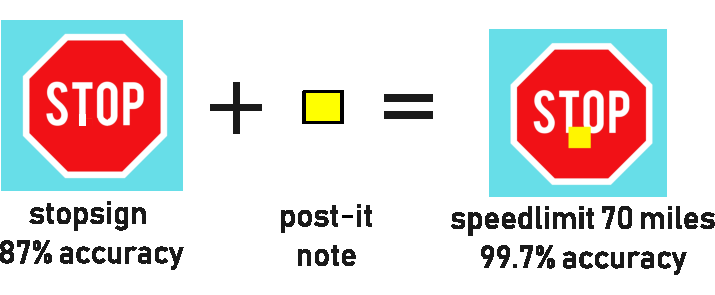
\includegraphics[width=.8\textwidth]{img/fooling-signs.pdf}
	\vfill
	\vspace{-1em}
	\begin{quote}
		\tiny Eykholt, K., Evtimov, I., Fernandes, E., Li, B., Rahmati, A., Xiao, C., ... \& Song, D. (2018). Robust physical-world attacks on deep learning visual classification. In Proceedings of the IEEE conference on computer vision and pattern recognition (pp. 1625-1634).
		
	\end{quote}
\end{frame}

%%%%%%%%%%%%%%%%%%%%%%%%%%%%%%%%%%%%%%%%%%%%%%%%%%%%%%%%%%%%
\begin{frame}
\frametitle{EVEN MORE REASONS! (NLP)**}
\begin{columns}[c]
    \begin{column}{.5\textwidth}
    \Large

        \begin{itemize}
        \Large
            \item {Adversarial examples in NLP}
            \begin{itemize}
                    \Large

                \item Character perturbations
                \item Word perturbations
                \item Sentence perturbations
            \end{itemize}
            % \item Critical applications
            % \begin{itemize}
            %     \item Legal - to abide legislation
            %     \item Safety - for example in the medical field
            % \end{itemize}
        \end{itemize}
        
    \end{column}
    \begin{column}{.5\textwidth}
    \Large

    \begin{center}
        \textcolor{aisecpurple}{Are you a robot?}\\
    \end{center}
    \end{column}
\end{columns}
\vfill
	\begin{quote}
		\tiny Casadio, M., {{Arnaboldi, L.}}, Daggitt, M. L., Isac, O., Dinkar, T., Kienitz, D., ... \& Komendantskaya, E. (2023). ANTONIO: Towards a Systematic Method of Generating NLP Benchmarks for Verification. arXiv preprint arXiv:2305.04003.
		
	\end{quote}
 \vfill
 \tiny {\textbf{**With slide contributions from M. Casadio (Thanks)**}}
\end{frame}
%%%%%%%%%%%%%%%%%%%%%%%%%%%%%%%%%%%%%%%%%%%%%%%%%%%%%%%%%%%%
\begin{frame}
\frametitle{EVEN MORE REASONS! (NLP)}

\begin{columns}[c]
    \begin{column}{.5\textwidth}    \Large

        \begin{itemize}
            \item Adversarial examples in NLP
            \begin{itemize}    \Large

                \item \textcolor{aisecred}{Character perturbations}
                \item Word perturbations
                \item Sentence perturbations
            \end{itemize}
            % \item Critical applications
            % \begin{itemize}
            %     \item Legal - to abide legislation
            %     \item Safety - for example in the medical field
            % \end{itemize}
        \end{itemize}
    \end{column}
    \begin{column}{.5\textwidth}
    \begin{center}    \Large

        \textcolor{aisecpurple}{Are you a robot?}\\
        \textcolor{aisecpurple}{Are you a r}\textcolor{aisecred}{p}\textcolor{aisecpurple}{bot?}\\
        \textcolor{aisecpurple}{Are you a}\textcolor{aisecred}{n }\textcolor{aisecpurple}{robot?}
    \end{center}
    \end{column}
\end{columns}
\vfill
	\begin{quote}
		\tiny Casadio, M., \textbf{\textbf{Arnaboldi, L.}}, Daggitt, M. L., Isac, O., Dinkar, T., Kienitz, D., ... \& Komendantskaya, E. (2023). ANTONIO: Towards a Systematic Method of Generating NLP Benchmarks for Verification. arXiv preprint arXiv:2305.04003.
		
	\end{quote}
\end{frame}

%%%%%%%%%%%%%%%%%%%%%%%%%%%%%%%%%%%%%%%%%%%%%%%%%%%%%%%%%%%%
\begin{frame}
\frametitle{EVEN MORE REASONS! (NLP)}

\begin{columns}[c]
    \begin{column}{.5\textwidth}
        \begin{itemize}    \Large

            \item Adversarial examples in NLP
            \begin{itemize}    \Large

                \item Character perturbations
                \item \textcolor{aisecred}{Word perturbations}
                \item Sentence perturbations
            \end{itemize}
            % \item Critical applications
            % \begin{itemize}
            %     \item Legal - to abide legislation
            %     \item Safety - for example in the medical field
            % \end{itemize}
        \end{itemize}
    \end{column}
    \begin{column}{.5\textwidth}
    \begin{center}    \Large

        \textcolor{aisecpurple}{Are you a robot?}\\
        \textcolor{aisecpurple}{Are you }\textcolor{aisecred}{not }\textcolor{aisecpurple}{a robot?}\\
        \textcolor{aisecred}{Were }\textcolor{aisecpurple}{you a robot?}
    \end{center}
    \end{column}
\end{columns}
\vfill
	\begin{quote}
		\tiny Casadio, M., {{Arnaboldi, L.}}, Daggitt, M. L., Isac, O., Dinkar, T., Kienitz, D., ... \& Komendantskaya, E. (2023). ANTONIO: Towards a Systematic Method of Generating NLP Benchmarks for Verification. arXiv preprint arXiv:2305.04003.
		
	\end{quote}
\end{frame}
%%%%%%%%%%%%%%%%%%%%%%%%%%%%%%%%%%%%%%%%%%%%%%%%%%%%%%%%%%%%
\begin{frame}
\frametitle{EVEN MORE REASONS! (NLP)}

\begin{columns}[c]
    \begin{column}{.5\textwidth}
        \begin{itemize}    \Large

            \item Adversarial examples in NLP
            \begin{itemize}    \Large

                \item Character perturbations
                \item Word perturbations
                \item \textcolor{aisecred}{Sentence perturbations}
            \end{itemize}
            % \item Critical applications
            % \begin{itemize}
            %     \item Legal - to abide legislation
            %     \item Safety - for example in the medical field
            % \end{itemize}
        \end{itemize}
    \end{column}
    \begin{column}{.5\textwidth}
    \begin{center}    \Large

        \textcolor{aisecpurple}{Are you a robot?}\\
        \textcolor{aisecred}{Am I talking to }\textcolor{aisecpurple}{a robot?}\\
        \textcolor{aisecred}{Can u tell me if you are a chatbot?}
    \end{center}
    \end{column}
\end{columns}
\vfill
	\begin{quote}
		\tiny Casadio, M., {{Arnaboldi, L.}}, Daggitt, M. L., Isac, O., Dinkar, T., Kienitz, D., ... \& Komendantskaya, E. (2023). ANTONIO: Towards a Systematic Method of Generating NLP Benchmarks for Verification. arXiv preprint arXiv:2305.04003.
		
	\end{quote}
\end{frame}

\begin{frame}
\frametitle{Legal Requirement of NLP Verification}

    \begin{quote}
        \textcolor{aisecpurple}{People have the right to know if and when they are interacting with a machine’s algorithm instead of a human being, the AI Act introduces specific transparency obligations for both users and providers of AI system, such as bot disclosure. Limited Risk AI Systems such as chatbots necessitate specific transparency obligations as well [EU Legislation 2020]}

    \end{quote}

\end{frame}
% \begin{frame}[fragile]{EVEN MORE REASONS!}
% hi
% \end{frame}


\begin{frame}[fragile]{..... Yet another one? (Malware Analysis)}
\begin{columns}
    
\begin{column}{.5\textwidth}
 \textcolor{aisecred}{\textbf{BEFORE}}
        % \centering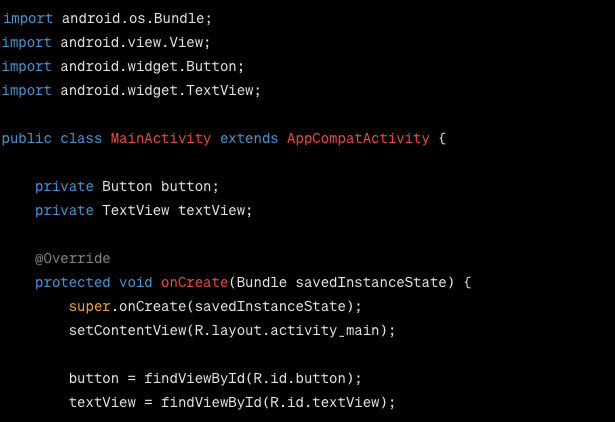
\includegraphics[width=\textwidth]{img/before.png}
\
        \begin{lstlisting}[language=java,basicstyle=\tiny,numbers=left]
import android.os.Bundle;
import android.view.View;
import android.widget.Button;
import android.widget.TextView;

public class MainActivity extends AppCompatActivity {

    private Button button;
    private TextView........
    ...
        \end{lstlisting}
    \end{column}
    \begin{column}{.5\textwidth}
 \textcolor{aisecred}{\textbf{AFTER}}
                \begin{lstlisting}[language=java,basicstyle=\tiny,numbers=left]]
import android.os.Bundle;
import android.view.View;
import android.widget.Button;
import android.widget.TextView;
import androidx.appcompat.app.AppCompatActivity;
import com.example.randomlibrary1.RandomLibrary1;
import com.example.randomlibrary2.RandomLibrary2;

public class MainActivity extends AppCompatActivity {

    private Button button;
    private TextView........
    ...
        \end{lstlisting}
    \end{column}
\end{columns}
lines \textbf{5} to \textbf{7} (AFTER)....
\vfill
	\begin{quote}
		\tiny Pierazzi, F., Pendlebury, F., Cortellazzi, J., \& Cavallaro, L. (2020, May). Intriguing properties of adversarial ml attacks in the problem space. In 2020 IEEE symposium on security and privacy (SP) (pp. 1332-1349). IEEE.
		
	\end{quote}
\end{frame}


\begin{frame}[fragile]{OK - I promise last one! (ML Network IDS)}
    \begin{itemize}
        \item Identification fields: Src IP, Src Port, Dst IP,Dst Port, Protocol,Timestamp
        \item Features: Flow Duration, Fwd/Bwd Header Length, (Fwd/Bwd) Packet Length Min/Max/Mean/Std/Total, Total Fwd/Bwd Packets, (Fwd/Bwd) Inter- Arrival Time Min/Max/Mean/Std/Total, (Fwd/Bwd) SYN/FIN/ACK/RST/CWR/PSH/URG/ECE flags count, Packets/second, Bytes/second, Flow Active Duration Min/Max/Mean/Std, Subflow (Fwd/Bwd) Packets/Bytes, Up/Down Ratio
        \item Label: FlowType (should be mapped to 0 - BENIGN or 1 - MALICIOUS)
        \item \textbf{\textcolor{aisecred}{Attacker Objective:}} Can packets be manypulated in such a way that the classifcation switches?
        % \item \textbf{\textcolor{aisecred}{Objective:}} Given an attacker can perturb these, can we still correctly classify benign and malign traffic?

    \end{itemize}
    
    \begin{quote}\tiny
Apruzzese, G., Andreolini, M., Ferretti, L., Marchetti, M., \& Colajanni, M. (2022). Modeling realistic adversarial attacks against network intrusion detection systems. Digital Threats: Research and Practice (DTRAP), 3(3), 1-19.
	 \end{quote}
    

	% \begin{quote}
	% 	\tiny Panchuk, B., \textbf{Arnaboldi, L.}, Daggitt, K., \& Letychevskyi, O. (2023, Coming Soon). Formal Verification of ML Based Network Intrusion Detection. Work in progress
		
	% \end{quote}

    
\end{frame}

% \begin{frame}[fragile]{OH and there is this thing...}
% hi
% \end{frame}

\begin{frame}{Summary so far}

\begin{columns}
\begin{column}{0.3\textwidth}

\centering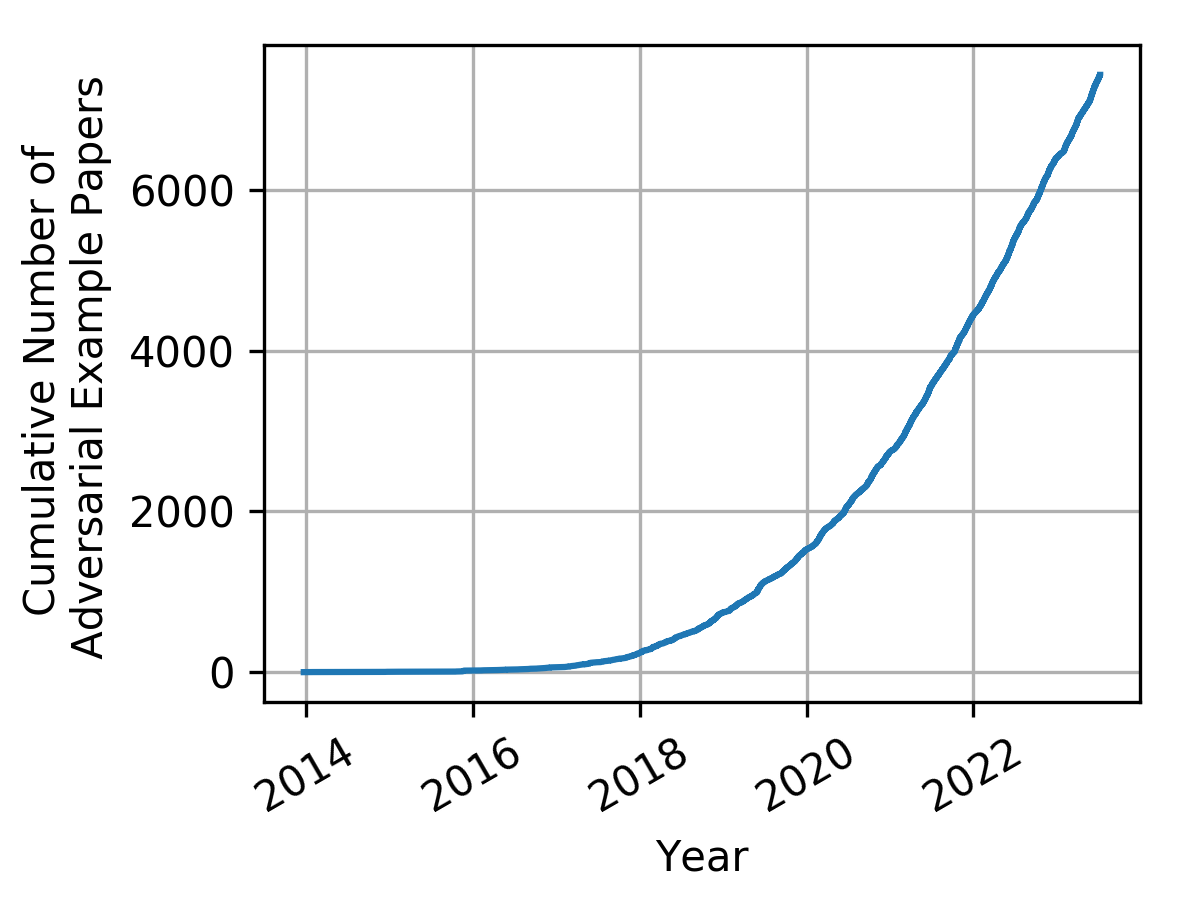
\includegraphics[width=1.3\textwidth]{img/amount-of-papers.png}
   
\end{column}
\begin{column}{0.60\textwidth}  %%<--- here
    \begin{itemize}
       \item Adversarial attacks are here to stay
       \item Verification is a promising way to protect against them
       \item We have a tool to specify properties and verify them
       \item So what are the open problems?
       \item .... \textbf{Remember NLP? (Malware, Text, Dialogue etc....}
   \end{itemize}
\end{column}
\end{columns}
\end{frame}

% \begin{frame}

% \frametitle{NLP Verification - Our approach}
% NOT LLMs. (Too big) - Setup a filter network instead

% \vspace{1em}

%         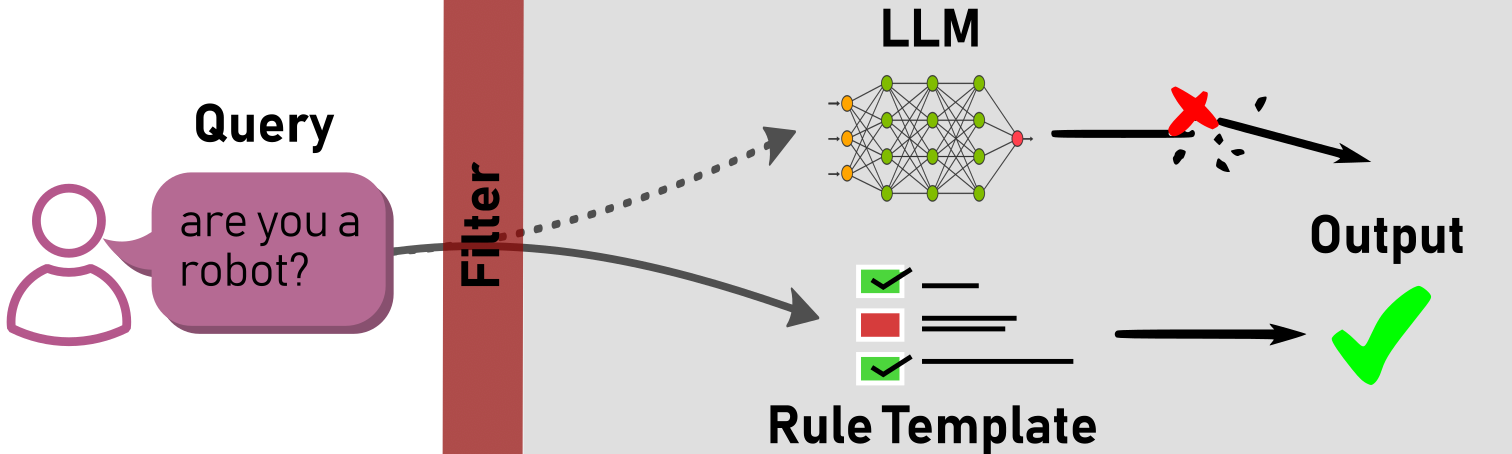
\includegraphics[width= \textwidth]{img/filter-broken.png}
% \end{frame}


% \begin{frame}
% \frametitle{NLP Verification - Our approach}

% \begin{columns}[c]
%     \begin{column}{.5\textwidth}
%         \begin{itemize}
%             \item \textcolor{aisecred}{Verify the NLP system}
%             \item $\epsilon$-ball
%             \item Naive approach ($\epsilon$-ball verification)
%         \end{itemize}
%     \end{column}
%     \begin{column}{.5\textwidth}
%         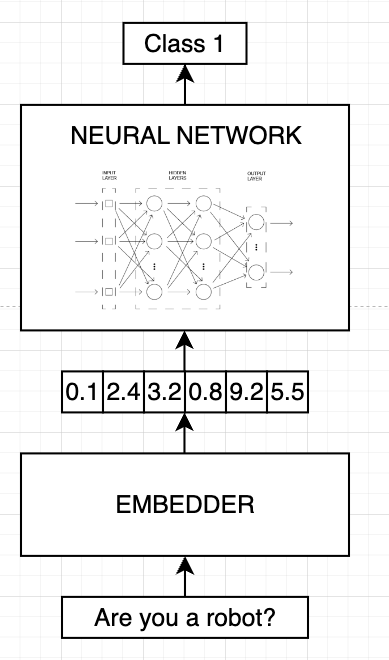
\includegraphics[width=0.5\textwidth]{img/nlpworkflow5.png}
%     \end{column}
% \end{columns}

% \end{frame}
% %%%%%%%%%%%%%%%%%%%%%%%%%%%%%%%%%%%%%%%%%%%%%%%%%%%%%%%%%%%%

% % \begin{frame}
% % \frametitle{NLP Verification - Our approach}

% % \begin{columns}[c]
% %     \begin{column}{.5\textwidth}
% %         \begin{itemize}
% %             \item \textcolor{aisecred}{Verify the \sout{NLP system} NN}
% %             \item $\epsilon$-ball
% %             \item Naive approach ($\epsilon$-ball verification)
% %         \end{itemize}
% %     \end{column}
% %     \begin{column}{.5\textwidth}
% %         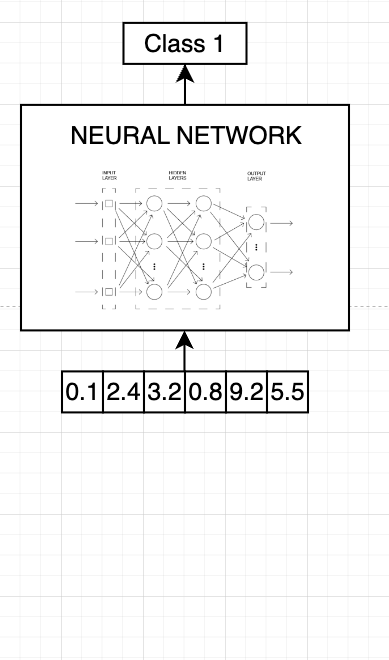
\includegraphics[width=0.5\textwidth]{img/nlpworkflow6.png}
% %     \end{column}
% % \end{columns}

% % \end{frame}
% % %%%%%%%%%%%%%%%%%%%%%%%%%%%%%%%%%%%%%%%%%%%%%%%%%%%%%%%%%%%%
% % \begin{frame}
% % \frametitle{NLP Verification - Our approach}

% % \begin{columns}[c]
% %     \begin{column}{.5\textwidth}
% %         \begin{itemize}
% %             \item Verify the neural network
% %             \item \textcolor{aisecred}{$\epsilon$-ball}
% %             \item Naive approach ($\epsilon$-ball verification)
% %         \end{itemize}
% %     \end{column}
% %     \begin{column}{.5\textwidth}
% %         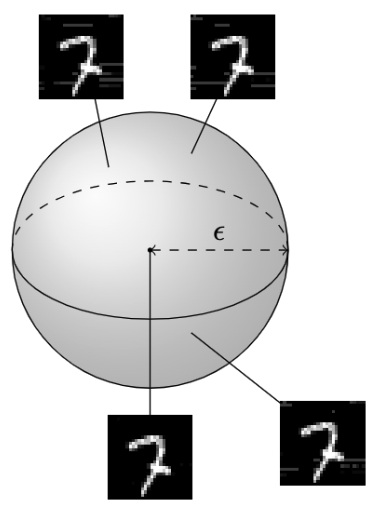
\includegraphics[width=0.5\textwidth]{img/epsballmnist.png}
% %     \end{column}
% % \end{columns}

% % \end{frame}
% % %%%%%%%%%%%%%%%%%%%%%%%%%%%%%%%%%%%%%%%%%%%%%%%%%%%%%%%%%%%%
% % \begin{frame}
% % \frametitle{NLP Verification - Our approach}

% % \begin{columns}[c]
% %     \begin{column}{.5\textwidth}
% %         \begin{itemize}
% %             \item Verify the neural network
% %             \item $\epsilon$-ball
% %             \item \textcolor{aisecred}{Naive approach ($\epsilon$-ball verification)}
% %         \end{itemize}
% %     \end{column}
% %     \begin{column}{.5\textwidth}
% %         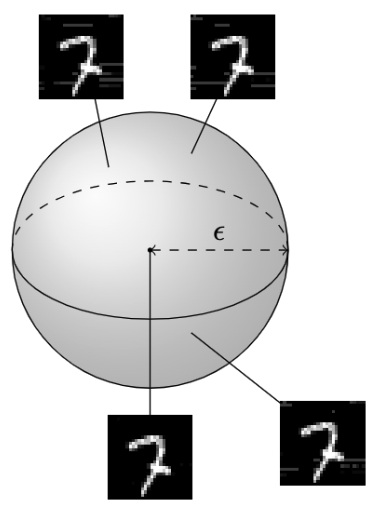
\includegraphics[width=0.5\textwidth]{img/epsballmnist.png}
% %     \end{column}
% % \end{columns}

% % \end{frame}
% % %%%%%%%%%%%%%%%%%%%%%%%%%%%%%%%%%%%%%%%%%%%%%%%%%%%%%%%%%%%%
% % %%%%%%%%%%%%%%%%%%%%%%%%%%%%%%%%%%%%%%%%%%%%%%%%%%%%%%%%%%%%
%  \begin{frame}


% \frametitle{NLP Verification -  Obstacles to Verification}

%    \begin{enumerate}
%    \Large
%        \item \textbf{Continuous vs discrete space} changes to sentences do not correspond linearly to changes in embedding
       
% %        The most obvious characteristic is the discrete nature of the space of NLU, while in vision the space is usually viewed as continuous. 
% % That is, given an image, an arbitrary small change to the pixel values is still an image. But if we make an arbitrary random change to a sentence it may or may not result in a sentence.
% % This particularly poses a challenge for the adversarial attacks and defences when transferred to NLU~\cite{lei2019discrete,zhang2019adversarial}, in the sense that simple gradient-based methods cannot be used.
% % To be able to use verifiers, however, we need a continuous space. Thus, we create an artificial one through sentence embeddings (Section~\ref{sec:section2}).

% \item \textbf{Perceptibility by humans.} semantic preservation in NLP vs Perceptibility of Image Space
% %On a related topic, one of the most impressive properties of adversarial attack in vision is that small perturbations of the image data which are imperceptible to humans are sufficient to deceive the model~\cite{szegedy2014intriguing}, while this can hardly be true for NLU attacks. Instead of being imperceptible, the adversarial attacks in NLU typically are bounded by the fact that the semantics of the sentences is not altered (despite being perceptible). Whether the meaning is changed or not largely depends on the human understanding of the sentence~\cite{minervini2018adversarially}. On the other hand, there are ways to generate samples where the changes, although being perceptible, are often ignored by human brain due to psychological biases on how a human processes the text~\cite{anastasopoulos2019neural,wang2020word}.

% \item \textbf{Difference of the data support.} from range of pixels (RGB 255) to variety of embedders
% %Another difference is in the domain adaptation for CV and NLU. In vision, although the images from the training and test distributions will be different, the distributions mostly share the same support (the pixels are always sample from a 0-255 integer space). On the other hand, in NLU the supports of the data often differ (e.g., the vocabularies can be significantly different in cross-lingual study~\cite{abad2019cross,zhang-etal-2020-margin}).

% % \textbf{Range of verification properties.} 
% % %Additionally, the majority of work on verification focuses on robustness properties of \emph{$\epsilon$-balls} around inputs, defined as 
% % $\mathbb{B}({\hat{\mathbf{x}}}, {\epsilon}) \triangleq \{\mathbf{x} \in \mathbb{R}^n \mid | {\mathbf{x}} - {\hat{\mathbf{x}}} |_{l_\infty} \leq \epsilon\}$
% % where  $\hat{\mathbf{x}}$ is the original input and $\mathbf{x}$ is any point around it (Figure~\ref{fig:eball}).
% % An input is robust within the \emph{$\epsilon$-ball} for a network if, for any point in the \emph{$\epsilon$-ball}, the model's output remains the same as for the original input.
% % Usually, for a verifier to succeed to prove the property, the $\epsilon$ is rather small, for example, it is 0.1 for a network trained on the FASHION data set~\cite{CKDKKAE22}.
%    \end{enumerate}

% \end{frame}

% % \begin{frame}
% % \frametitle{NLP Verification - More Obstacles}

% % \begin{columns}[c]
% %     \begin{column}{.5\textwidth}
% %         There are some obstacles the prevent this naive method to be effective:
% %         \begin{itemize}
% %             \item $\epsilon$-balls may not contain valid sentences
% %             \item Semantic similarity does not entail geometric proximity [Pierazzi et al.]
% %             \item Generally, NNs need to be trained to satisfy logical/semantic properties
% %         \end{itemize}
% %     \end{column}
% %     \begin{column}{.5\textwidth}
% %         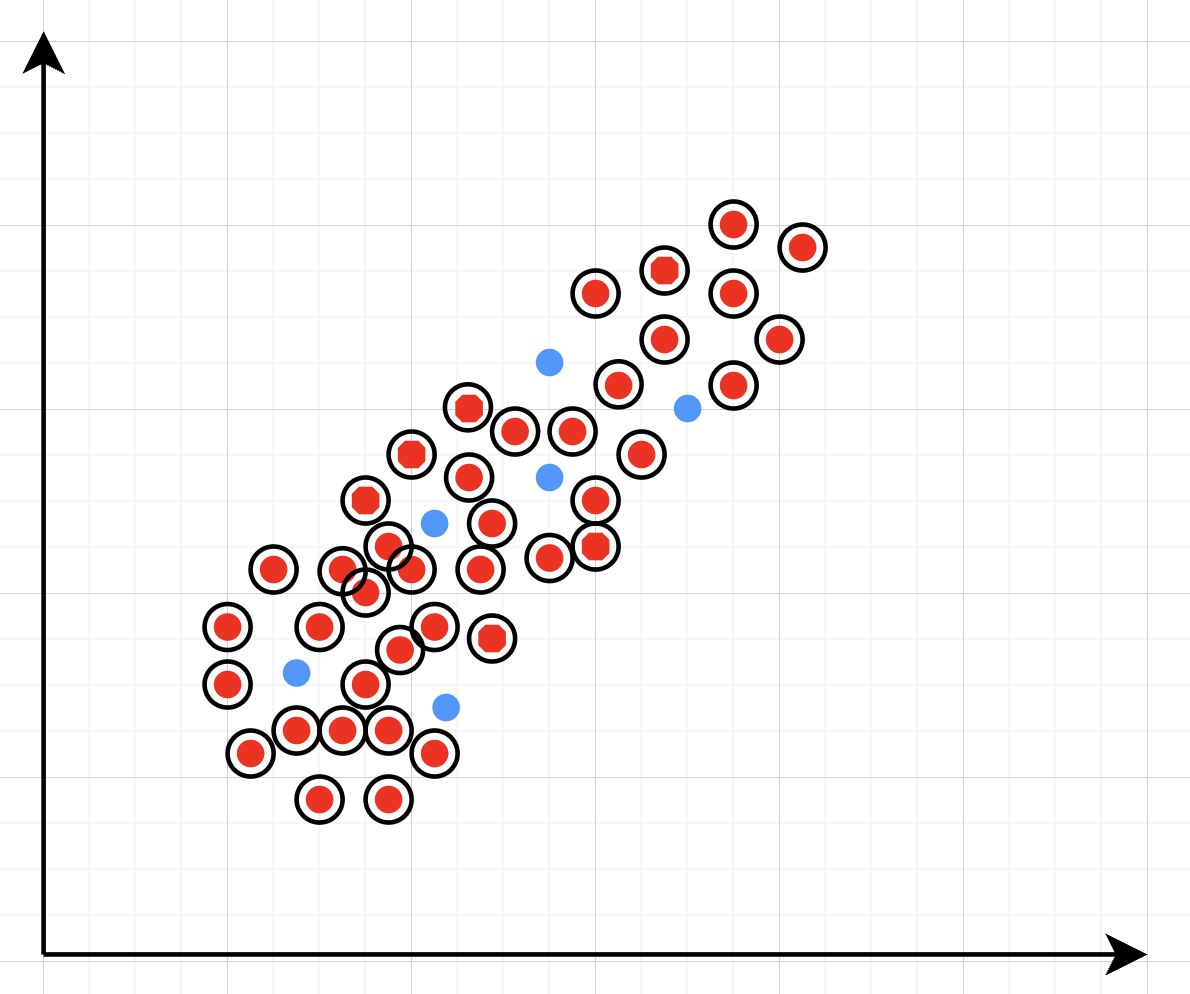
\includegraphics[width=0.8\textwidth]{img/eball.png}
% %     \end{column}
% % \end{columns}

% % \end{frame}


% % \begin{frame}
% % \frametitle{NLP Verification - Solutions}
% % \vspace{-1.5em}
% % \begin{columns}[c]
% %     \begin{column}{.5\textwidth}
% %         We propose some solutions:
% %         \begin{itemize}
% %             \item \textcolor{aisecred}{Hyper-rectangles}
% %             \begin{itemize}
% %                 \item Rotation
% %                 \item Shrinking
% %                 \item Clustering
% %             \end{itemize}
% %             \item Exploring spaces that cover semantic similarities
% %             \item Training networks to have more precise decision boundaries
% %             \begin{itemize}
% %                 \item Data augmentation
% %                 \item Adversarial training
% %             \end{itemize}
% %         \end{itemize}
% %     \end{column}
% %     \begin{column}{.5\textwidth}
% %     \begin{center}
% %         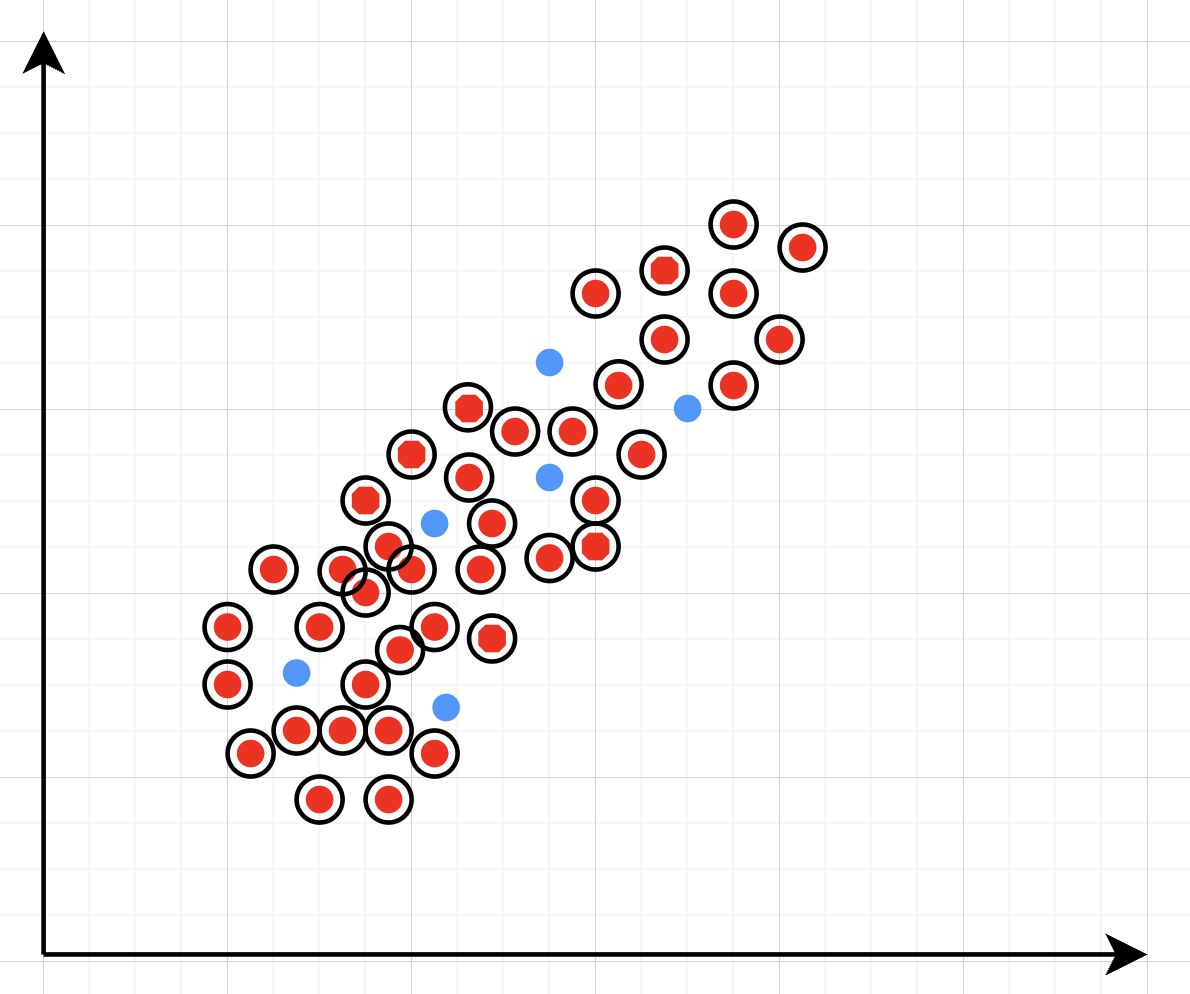
\includegraphics[width=0.5\textwidth]{img/eball.png}
% %         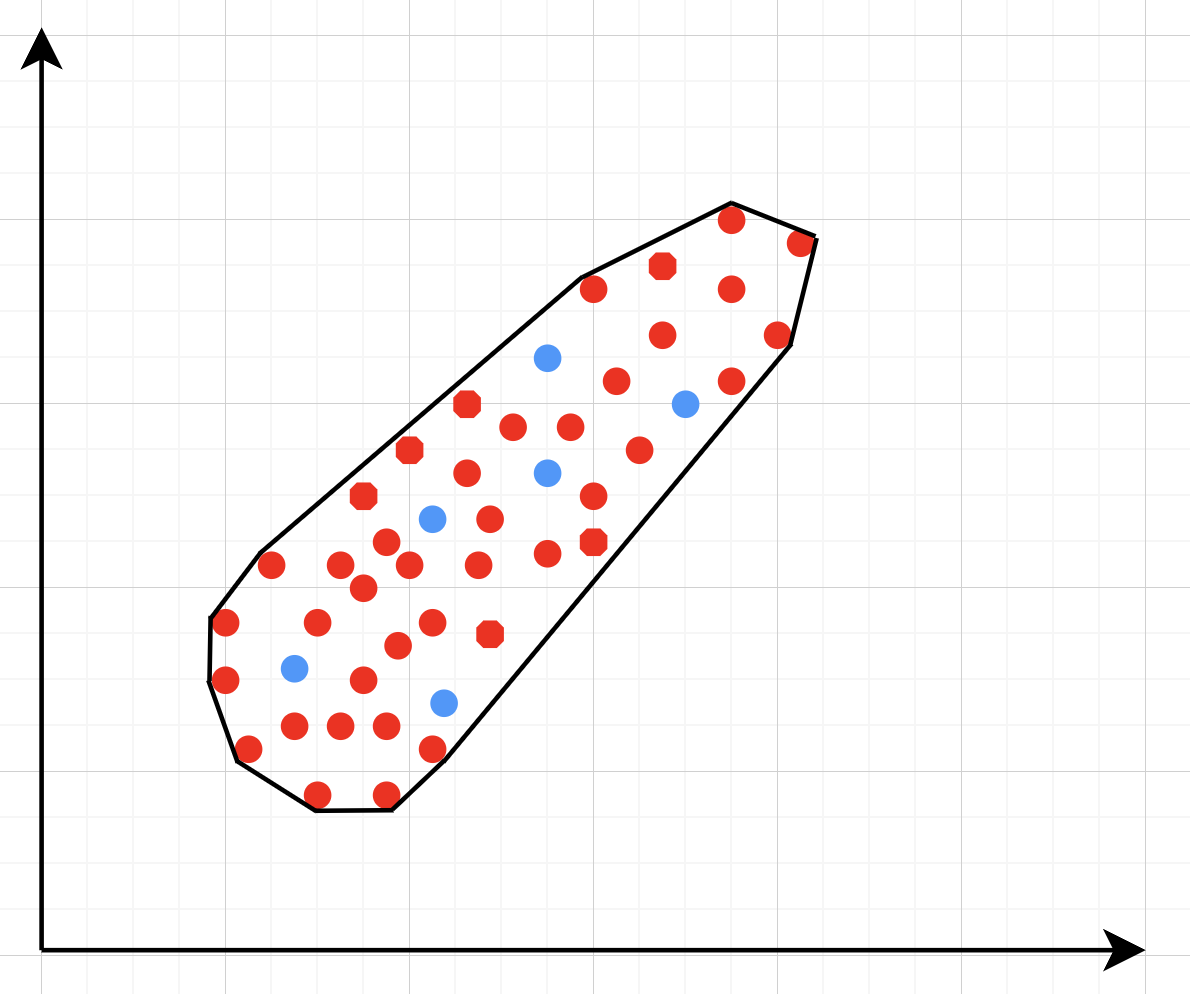
\includegraphics[width=0.5\textwidth]{img/convhull.png}
% %     \end{center}
% %     \end{column}
% % \end{columns}

% % \end{frame}
% % %%%%%%%%%%%%%%%%%%%%%%%%%%%%%%%%%%%%%%%%%%%%%%%%%%%%%%%%%%%%
% % \begin{frame}
% % \frametitle{Solutions}
% % \vspace{-1.5em}

% % \begin{columns}[c]
% %     \begin{column}{.5\textwidth}
% %         We propose some solutions:
% %         \begin{itemize}
% %             \item \textcolor{aisecred}{Hyper-rectangles}
% %             \begin{itemize}
% %                 \item Rotation
% %                 \item Shrinking
% %                 \item Clustering
% %             \end{itemize}
% %             \item Exploring spaces that cover semantic similarities
% %             \item Training networks to have more precise decision boundaries
% %             \begin{itemize}
% %                 \item Data augmentation
% %                 \item Adversarial training
% %             \end{itemize}
% %         \end{itemize}
% %     \end{column}
% %     \begin{column}{.5\textwidth}
% %     \begin{center}
% %         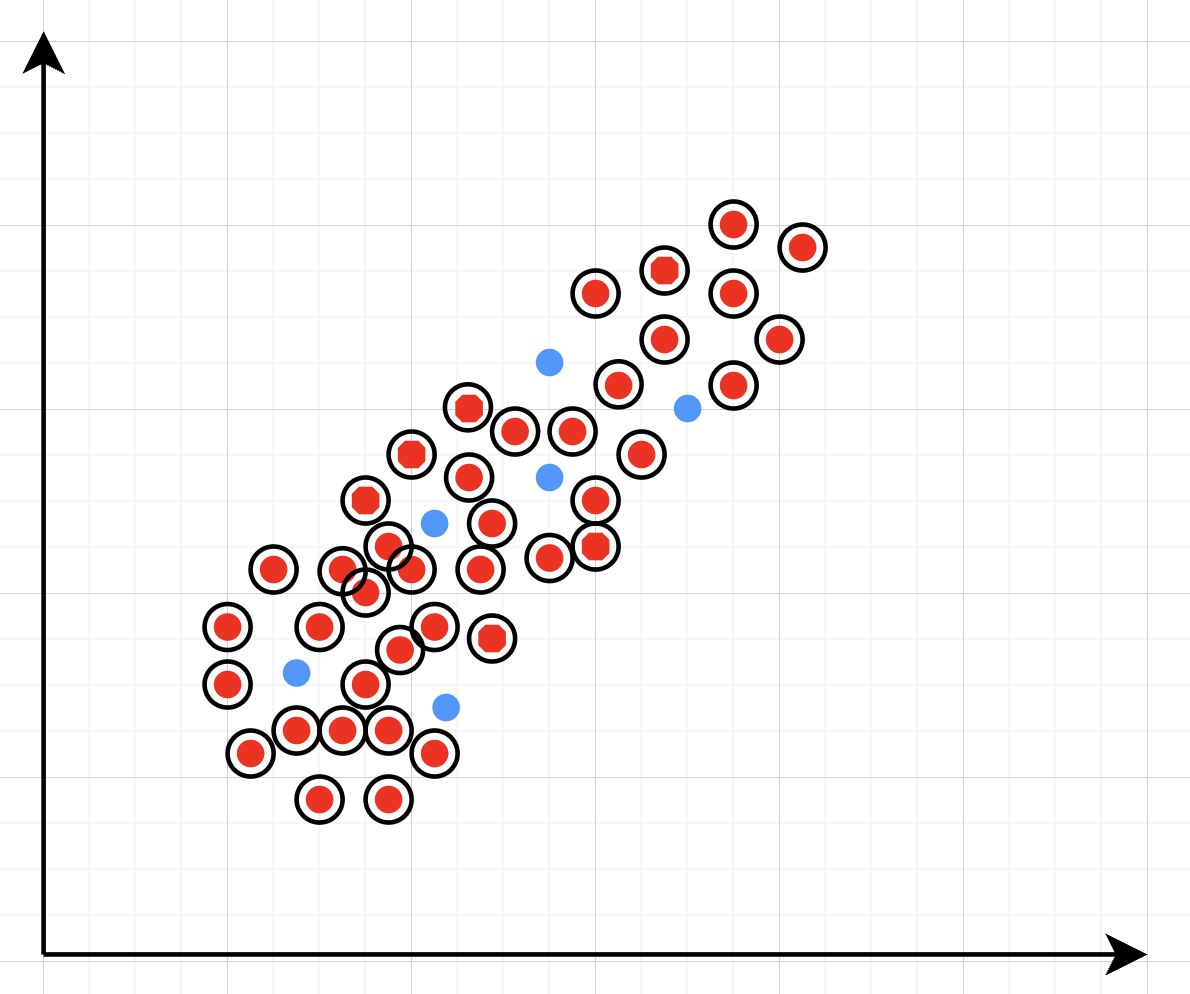
\includegraphics[width=0.5\textwidth]{img/eball.png}
% %         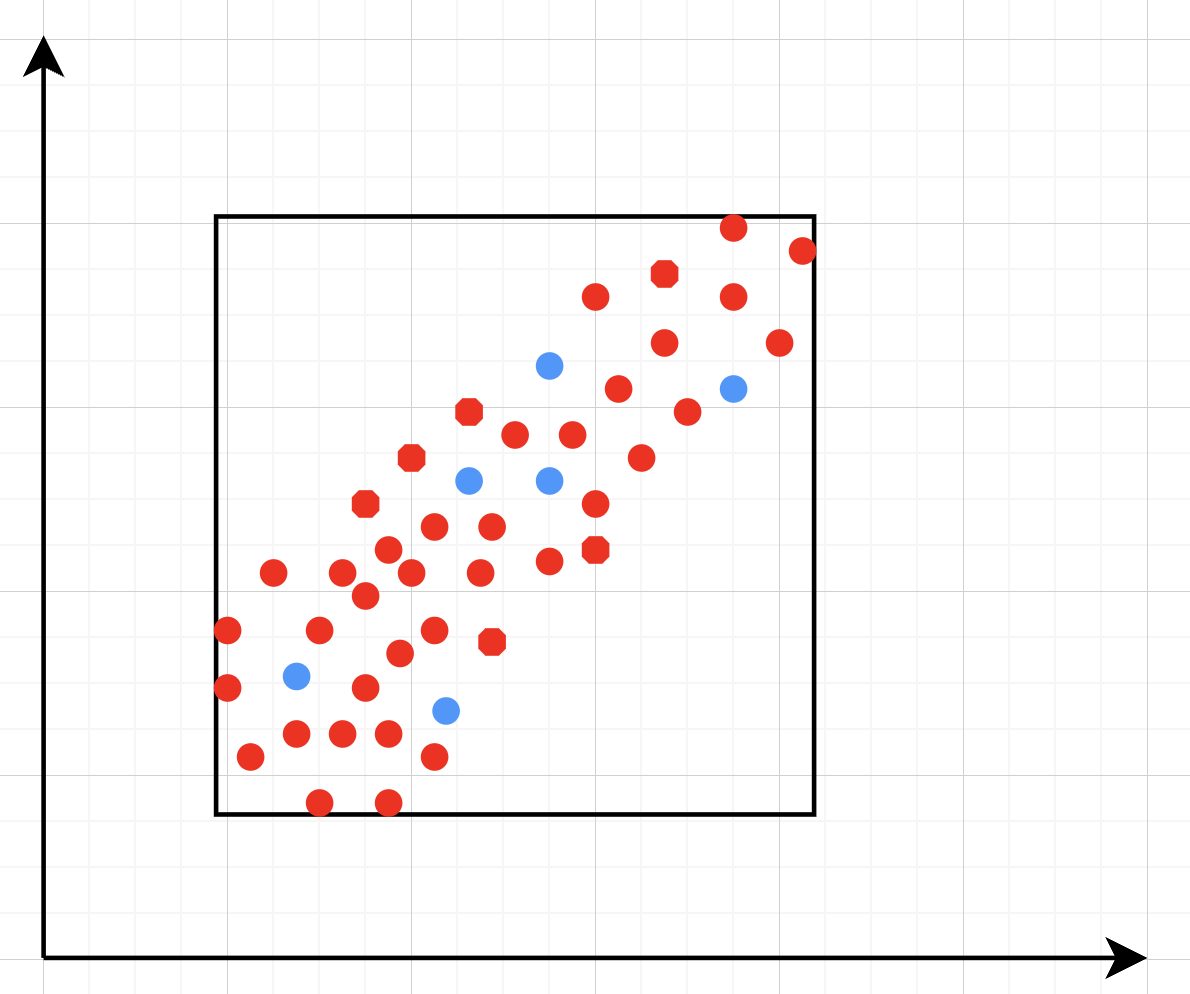
\includegraphics[width=0.5\textwidth]{img/hyperc.png}
% %     \end{center}
% %     \end{column}
% % \end{columns}

% % \end{frame}
% % %%%%%%%%%%%%%%%%%%%%%%%%%%%%%%%%%%%%%%%%%%%%%%%%%%%%%%%%%%%%
% % \begin{frame}
% % \frametitle{NLP Verification - Solutions}
% % \vspace{-1.5em}

% % \begin{columns}[c]
% %     \begin{column}{.5\textwidth}
% %         We propose some solutions:
% %         \begin{itemize}
% %             \item Hyper-rectangles
% %             \begin{itemize}
% %                 \item \textcolor{aisecred}{Rotation}
% %                 \item Shrinking
% %                 \item Clustering
% %             \end{itemize}
% %             \item Exploring spaces that cover semantic similarities
% %             \item Training networks to have more precise decision boundaries
% %             \begin{itemize}
% %                 \item Data augmentation
% %                 \item Adversarial training
% %             \end{itemize}
% %         \end{itemize}
% %     \end{column}
% %     \begin{column}{.5\textwidth}
% %     \begin{center}
% %         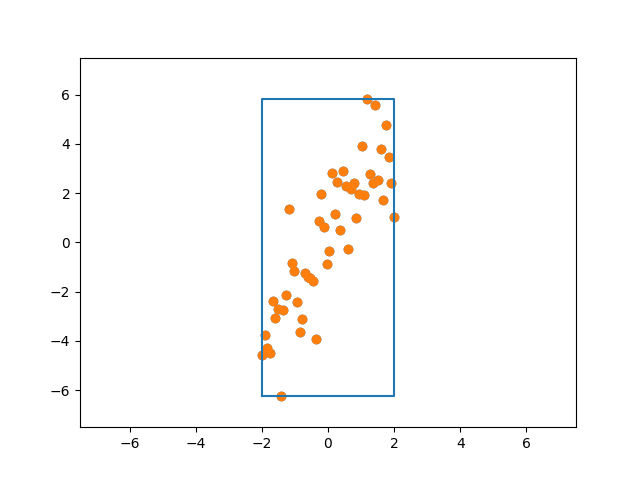
\includegraphics[width=0.5\textwidth]{img/original.png}
% %         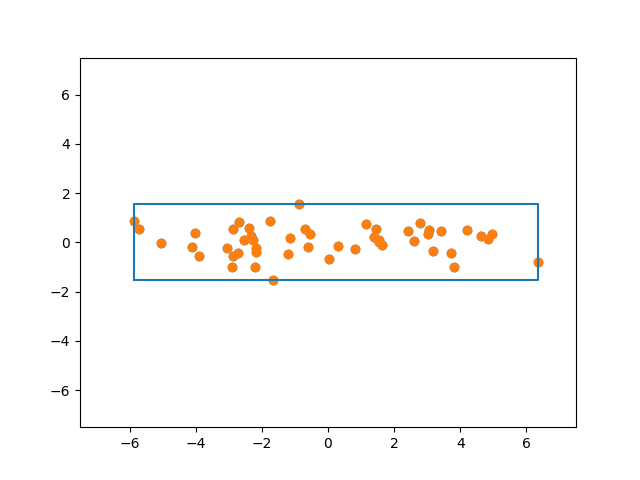
\includegraphics[width=0.5\textwidth]{img/rotated.png}
% %     \end{center}
% %     \end{column}
% % \end{columns}

% % \end{frame}
% % %%%%%%%%%%%%%%%%%%%%%%%%%%%%%%%%%%%%%%%%%%%%%%%%%%%%%%%%%%%%
% % \begin{frame}
% % \frametitle{NLP Verification - Solutions}
% % \vspace{-1.5em}

% % \begin{columns}[c]
% %     \begin{column}{.5\textwidth}
% %         We propose some solutions:
% %         \begin{itemize}
% %             \item Hyper-rectangles
% %             \begin{itemize}
% %                 \item Rotation
% %                 \item \textcolor{aisecred}{Shrinking}
% %                 \item Clustering
% %             \end{itemize}
% %             \item Exploring spaces that cover semantic similarities
% %             \item Training networks to have more precise decision boundaries
% %             \begin{itemize}
% %                 \item Data augmentation
% %                 \item Adversarial training
% %             \end{itemize}
% %         \end{itemize}
% %     \end{column}
% %     \begin{column}{.5\textwidth}
% %     \begin{center}
% %         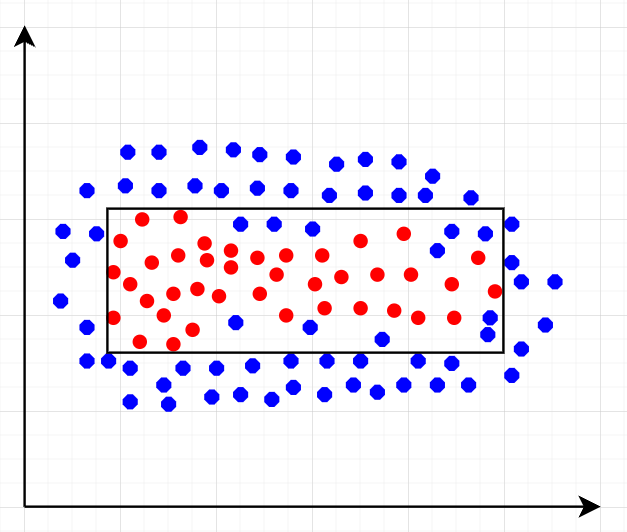
\includegraphics[width=0.5\textwidth]{img/rhyperc.png}
% %         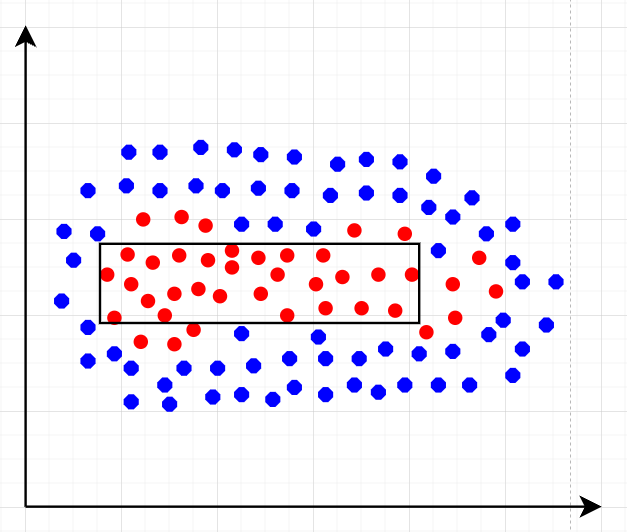
\includegraphics[width=0.5\textwidth]{img/rshyperc.png}
% %     \end{center}
% %     \end{column}
% % \end{columns}

% % \end{frame}
% % %%%%%%%%%%%%%%%%%%%%%%%%%%%%%%%%%%%%%%%%%%%%%%%%%%%%%%%%%%%%
% % \begin{frame}
% % \frametitle{NLP Verification - Solutions}
% % \vspace{-1.5em}

% % \begin{columns}[c]
% %     \begin{column}{.5\textwidth}
% %         We propose some solutions:
% %         \begin{itemize}
% %             \item Hyper-rectangles
% %             \begin{itemize}
% %                 \item Rotation
% %                 \item Shrinking
% %                 \item \textcolor{aisecred}{Clustering}
% %             \end{itemize}
% %             \item Exploring spaces that cover semantic similarities
% %             \item Training networks to have more precise decision boundaries
% %             \begin{itemize}
% %                 \item Data augmentation
% %                 \item Adversarial training
% %             \end{itemize}
% %         \end{itemize}
% %     \end{column}
% %     \begin{column}{.5\textwidth}
% %     \begin{center}
% %         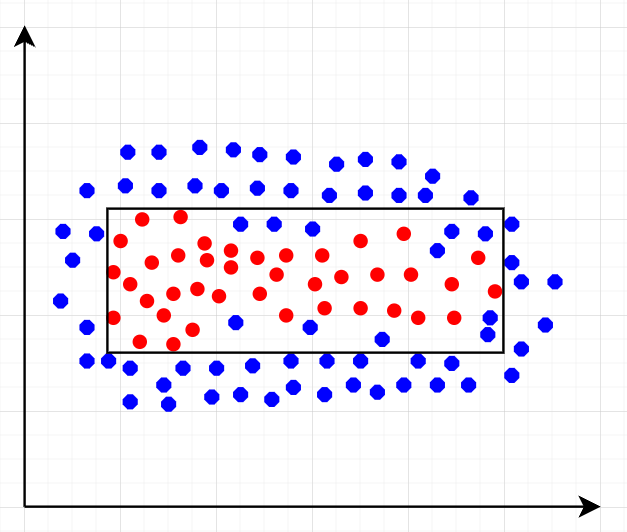
\includegraphics[width=0.5\textwidth]{img/rhyperc.png}
% %         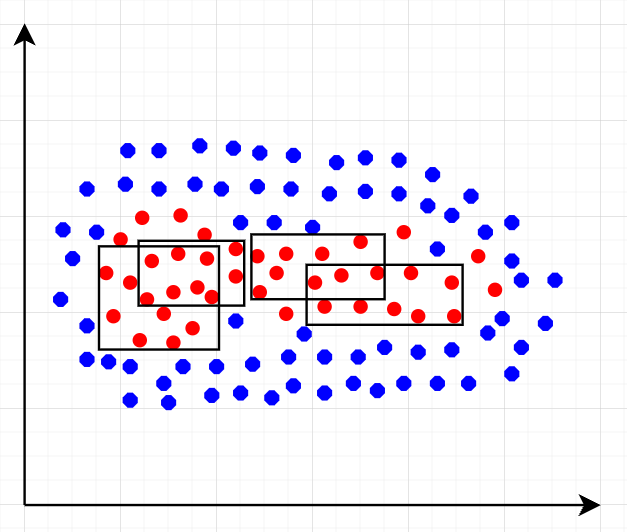
\includegraphics[width=0.5\textwidth]{img/rchyperc.png}
% %     \end{center}
% %     \end{column}
% % \end{columns}

% % \end{frame}
% % %%%%%%%%%%%%%%%%%%%%%%%%%%%%%%%%%%%%%%%%%%%%%%%%%%%%%%%%%%%%
% % \begin{frame}
% % \frametitle{NLP Verification - Solutions}
% % \vspace{-0em}

% % \begin{columns}[c]
% %     \begin{column}{.5\textwidth}
% %         We propose some solutions:
% %         \begin{itemize}
% %             \item Hyper-rectangles
% %             \begin{itemize}
% %                 \item Rotation
% %                 \item Shrinking
% %                 \item Clustering
% %             \end{itemize}
% %             \item \textcolor{aisecred}{Exploring spaces that cover semantic similarities}
% %             \item Training networks to have more precise decision boundaries
% %             \begin{itemize}
% %                 \item Data augmentation
% %                 \item Adversarial training
% %             \end{itemize}
% %         \end{itemize}
% %     \end{column}
% %     \begin{column}{.5\textwidth}
% %     \begin{center}
% %         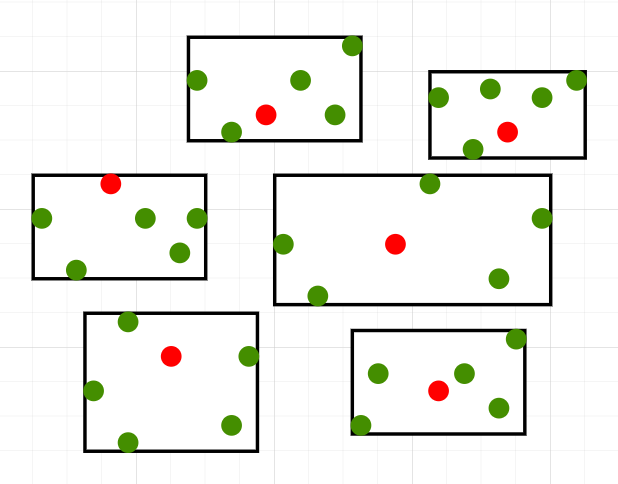
\includegraphics[width=0.9\textwidth]{img/cubeattack.png}
% %     \end{center}
% %     \end{column}
% % \end{columns}

% % \end{frame}
% % %%%%%%%%%%%%%%%%%%%%%%%%%%%%%%%%%%%%%%%%%%%%%%%%%%%%%%%%%%%%
% % \begin{frame}
% % \frametitle{NLP Verification - Solutions}

% % \begin{columns}[c]
% %     \begin{column}{.5\textwidth}
% %         We propose some solutions:
% %         \begin{itemize}
% %             \item Hyper-rectangles
% %             \begin{itemize}
% %                 \item Rotation
% %                 \item Shrinking
% %                 \item Clustering
% %             \end{itemize}
% %             \item Exploring spaces that cover semantic similarities
% %             \item \textcolor{aisecred}{Training networks to have more precise decision boundaries}
% %             \begin{itemize}
% %                 \item \textcolor{aisecred}{Data augmentation}
% %                 \item \textcolor{aisecred}{Adversarial training}
% %             \end{itemize}
% %         \end{itemize}
% %     \end{column}
% %     \begin{column}{.5\textwidth}
% %     \begin{center}
% %         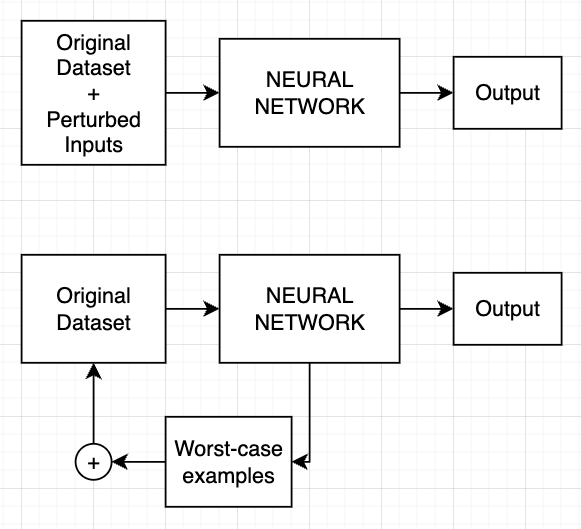
\includegraphics[width=0.9\textwidth]{img/robusttraining.png}
% %     \end{center}
% %     \end{column}
% % \end{columns}

% % \end{frame}
% %%%%%%%%%%%%%%%%%%%%%%%%%%%%%%%%%%%%%%%%%%%%%%%%%%%%%%%%%%%%
% %%%%%%%%%%%%%%%%%%%%%%%%%%%%%%%%%%%%%%%%%%%%%%%%%%%%%%%%%%%%
\begin{frame}
\frametitle{NLP Verification - ANTONIO}

\centering 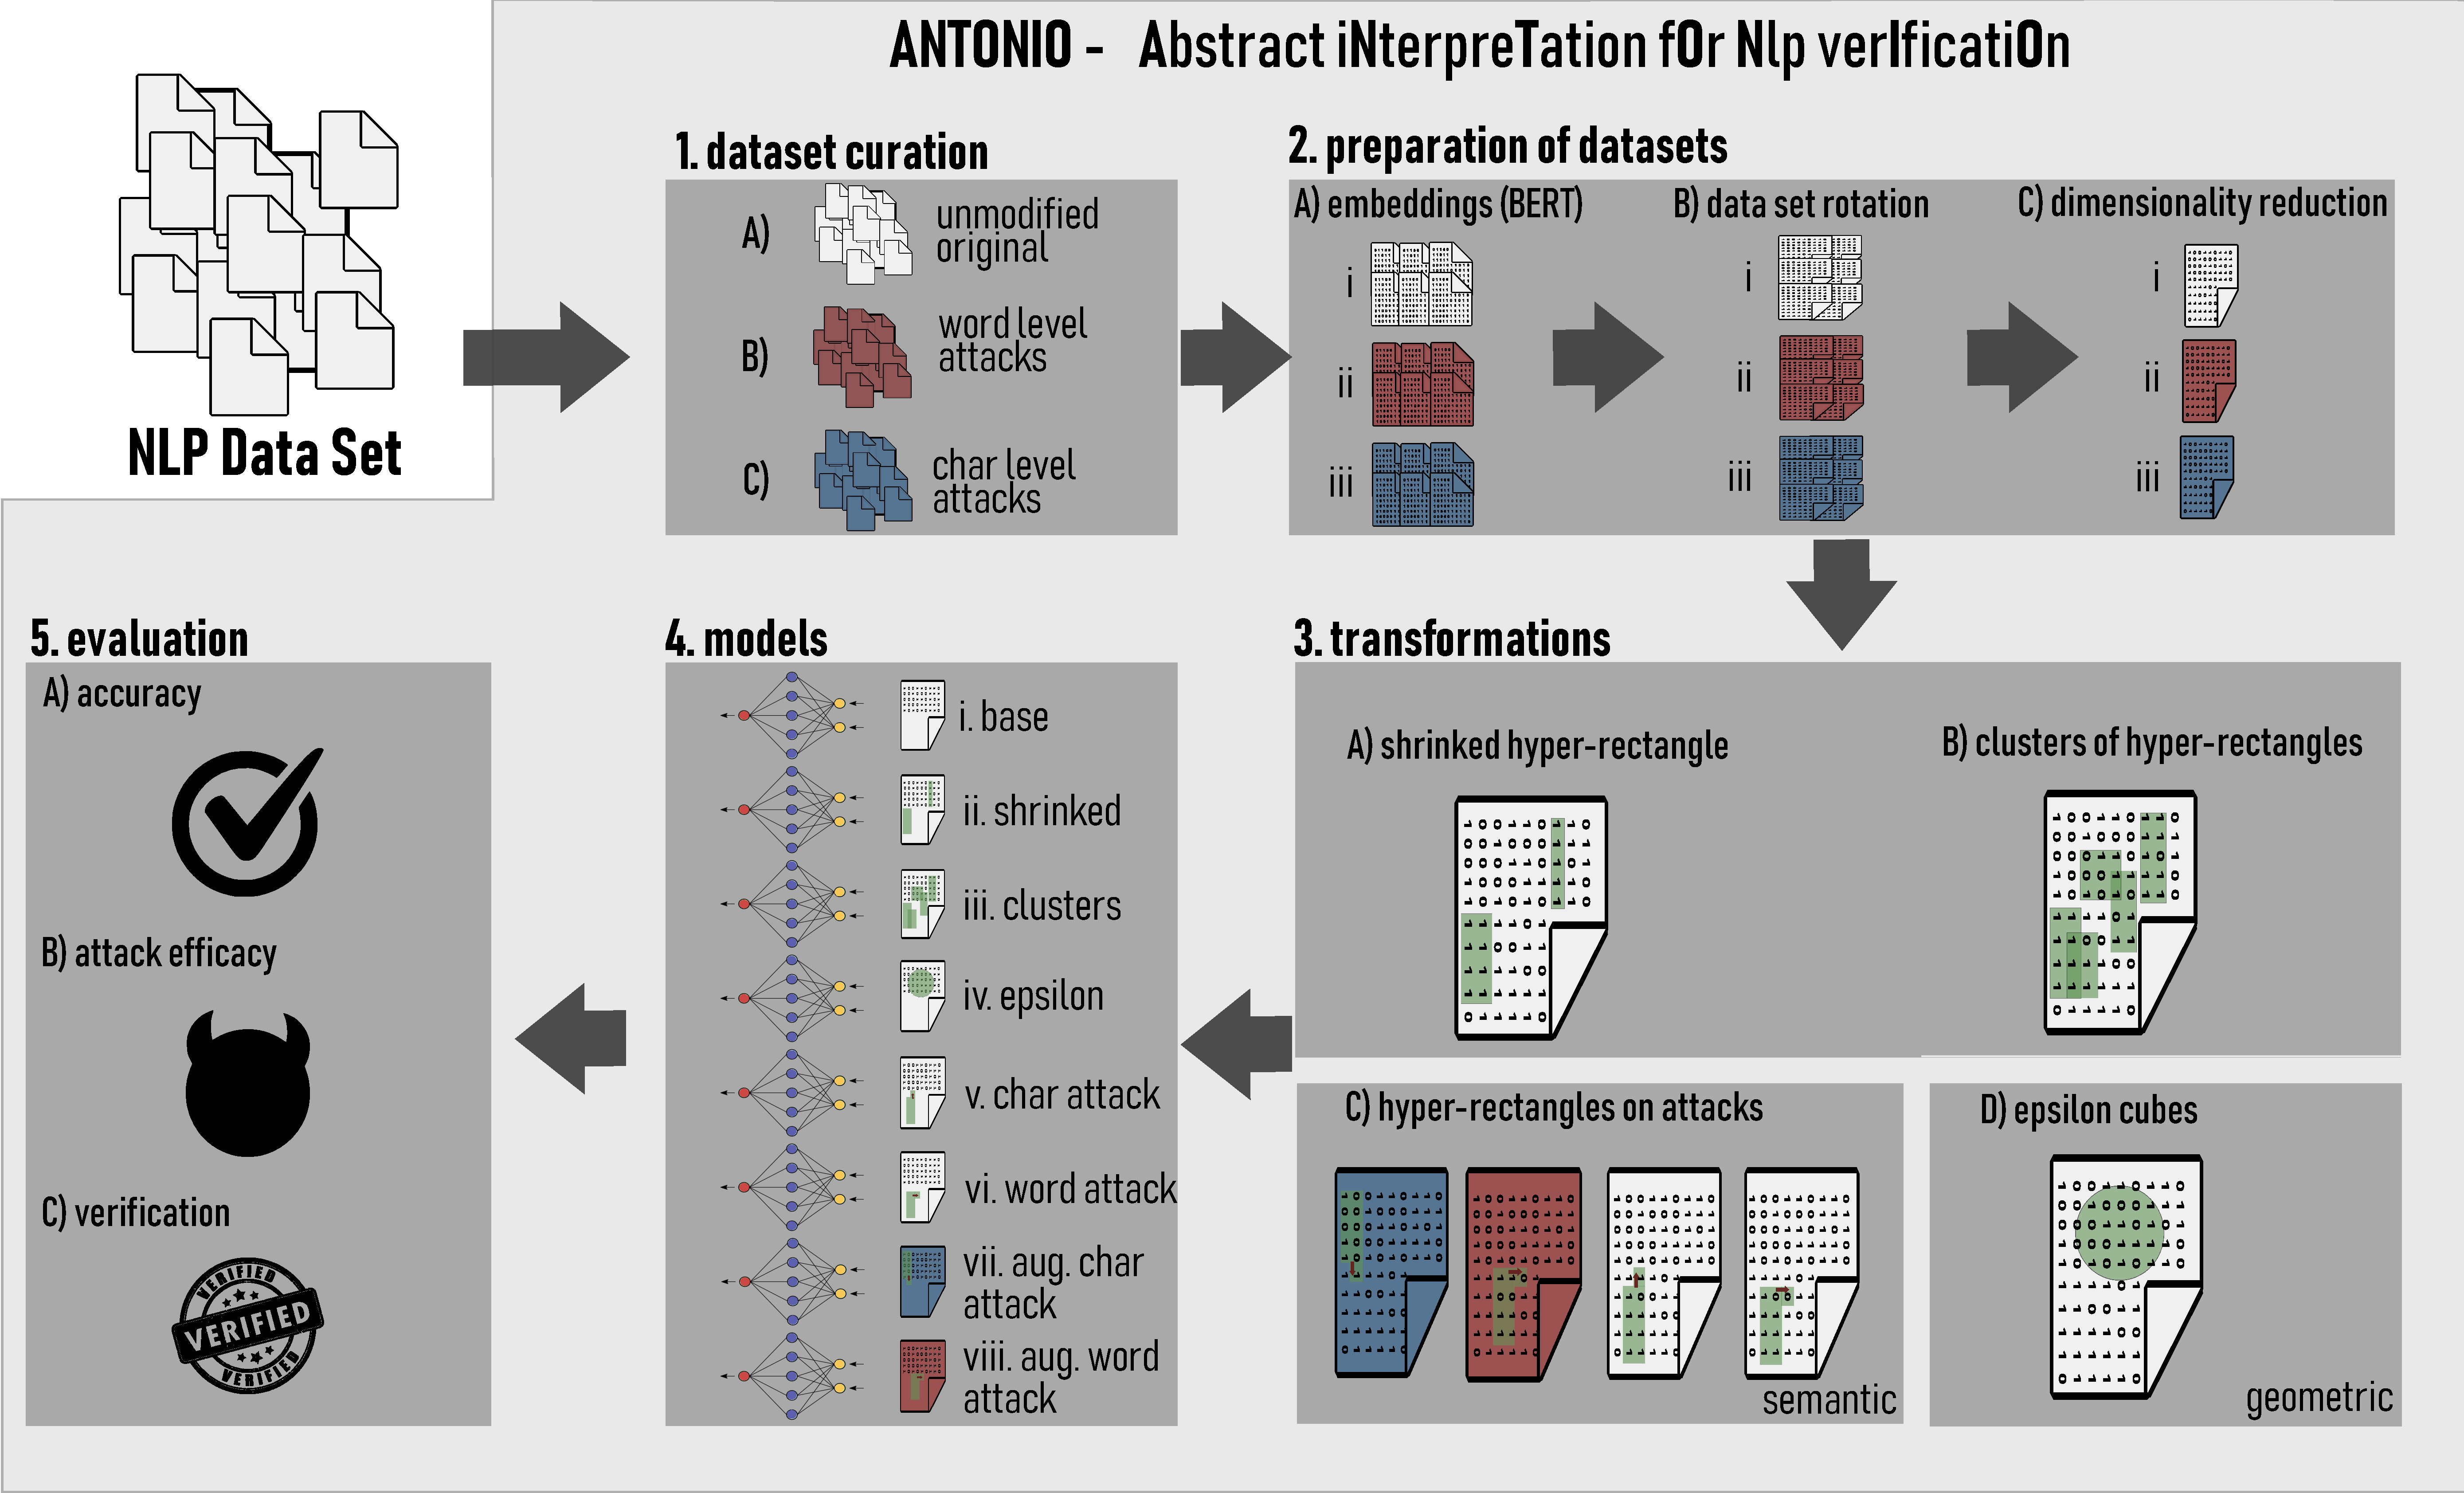
\includegraphics[width=0.75\textwidth]{img/ANTONIO-flow.pdf}

\end{frame}

% \begin{frame}
% \frametitle{NLP Verification - Results}
% \vspace{-1.5em}
% \begin{table}[h]
% \centering
% \begin{tabular}{|l|r|r|rrr|}
% \hline
% \multirow{2}{*}{\textbf{Model}} & \multirow{2}{*}{\textbf{Test Accuracy}} & \multirow{2}{*}{\textbf{Attack Accuracy}} &
%   \multicolumn{3}{c|}{\textbf{Verification}} \\ \cline{4-6}
%         &  &  & \multicolumn{1}{l|}{$\mathbb{H}_{\epsilon=0.005}$}& \multicolumn{1}{l|}{$\mathbb{H}_{\epsilon=0.05}$} & $\mathbb{H}_{pert}$ \\ \hline
% $N_{base}$ & \textbf{93.87} & 89.68     & \multicolumn{1}{r|}{88.67}  & \multicolumn{1}{r|} {1.79} &  11.69     \\ \hline
% $N_{adv}$ & 93.38 & \textbf{90.27} & \multicolumn{1}{r|} {\textbf{98.22}} & \multicolumn{1}{r|} {\textbf{12.17}}   &   \textbf{45.12}    \\ \hline
% \end{tabular}
% \caption{\emph{\footnotesize{Accuracy on test set and attacks and verificaton results using Marabou.}}}
% \end{table}

% \begin{table}[h]
% \centering
% \scriptsize
% \begin{tabular}{|l|r|r|r|r|}
% \hline
% \textbf{Hyper-rectangles} &  \textbf{Avg. Volume}&  \textbf{Contained U.S. (\%)} & \textbf{Contained U.S. (\#)} & \textbf{Total U.S.} \\
% \hline 
% $\mathbb{H}_{\epsilon=0.005}$ & 1.00e-60 & 1.95 & 2821 & 144500 \\
% $\mathbb{H}_{\epsilon=0.05}$ &1.00e-30 &38.47 & 55592 & 144500 \\
% $\mathbb{H}_{pert}$ & 1.28e-30 & \textbf{47.67} & \textbf{68882} & 144500 \\
% \hline
% \end{tabular}
% \caption{\emph{\footnotesize{Number of unseen sentences inside each collection of hyper-rectangles.}}}
% \end{table}

% \end{frame}

% \begin{frame}
% \frametitle{Results (for Are You A Robot? - Dataset [2021]}

% % Please add the following required packages to your document preamble:
% \begin{table}[]
% \centering
% \begin{tabular}{|l|l|l|lll|lll|}
% \hline
% \multirow{2}{*}{\textbf{Model}} & \multirow{2}{*}{\textbf{Accuracy}} & \multirow{2}{*}{\textbf{Attack Accuracy}} & \multicolumn{3}{l|}{\textbf{Verification (ERAN)}} &
%   \multicolumn{3}{l|}{\textbf{Verification (Marabou)}} \\ \cline{4-9}
%         &  &  & \multicolumn{1}{l|}{$\mathbb{H}^*_{250}$} & \multicolumn{1}{l|}{$\mathbb{H}^*_{\epsilon}$} & $\mathbb{H}^*_{word}$ & \multicolumn{1}{l|}{$\mathbb{H}^*_{250}$} & \multicolumn{1}{l|}{$\mathbb{H}^*_{\epsilon}$} & $\mathbb{H}^*_{word}$ \\ \hline
% $N_{base}$ & \textbf{93.87} & 89.68 & \multicolumn{1}{l|}{2.04}     & \multicolumn{1}{l|}{0}   &  0.94  & \multicolumn{1}{l|}{0.41}     & \multicolumn{1}{l|}{1.79}   &  11.69     \\ \hline
% $N_{\epsilon}$    & 93.48 & 90.17 & \multicolumn{1}{l|}{2.80}     & \multicolumn{1}{l|}{\textbf{0.36}}   & \textbf{8.08}  & \multicolumn{1}{l|}{\textbf{3.87}}     & \multicolumn{1}{l|}{\textbf{18.46}}   &   41.93    \\ \hline
% $N_{word}$ & 93.38 & \textbf{90.27} & \multicolumn{1}{l|}{\textbf{2.96}}     & \multicolumn{1}{l|}{\0}   &  6.04  & \multicolumn{1}{l|}{2.74}     & \multicolumn{1}{l|}{12.17}   &   \textbf{45.12}    \\ \hline
% \end{tabular}
% \end{table}

% \end{frame}

%\begin{frame}[fragile]{Attacks don't have to be sophisticated }
%	
% \hspace{1cm}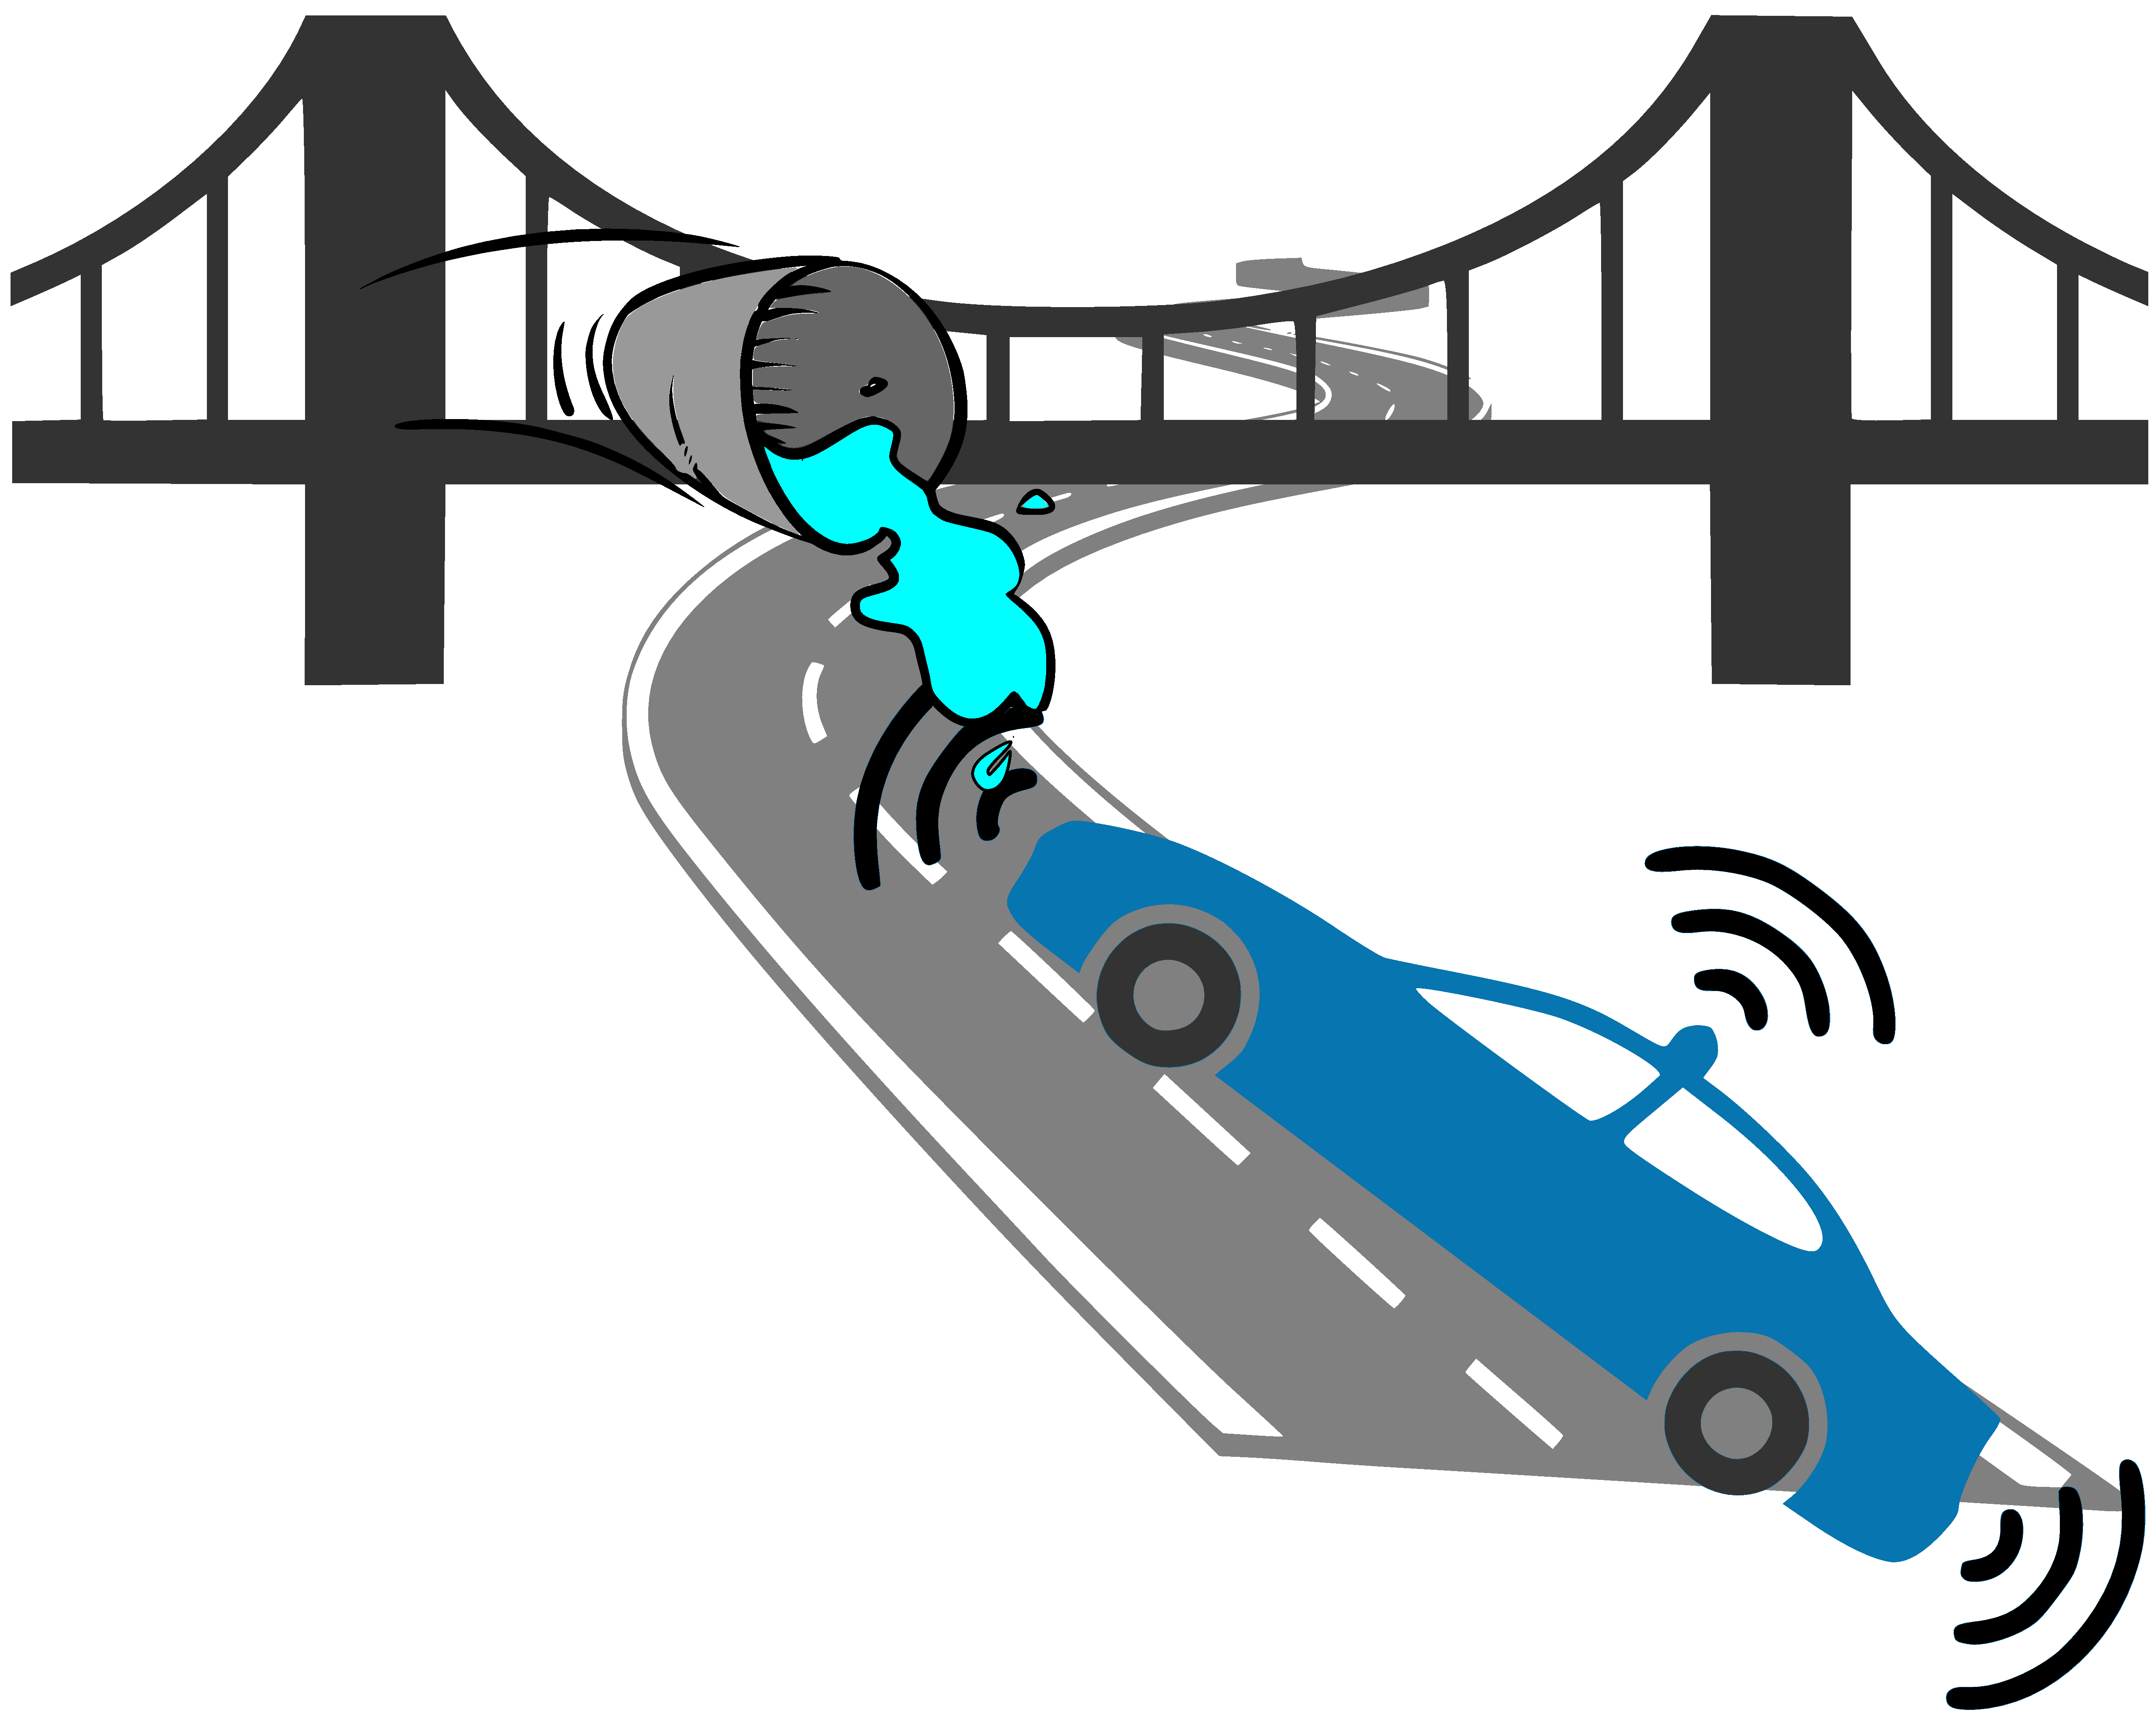
\includegraphics[width=.58\textwidth]{img/bucket-off-bridge.pdf}
%
%	
%\end{frame}

% \begin{frame}[fragile]{Attacks don't have to be sophisticated }
	
% 	\hspace{1cm}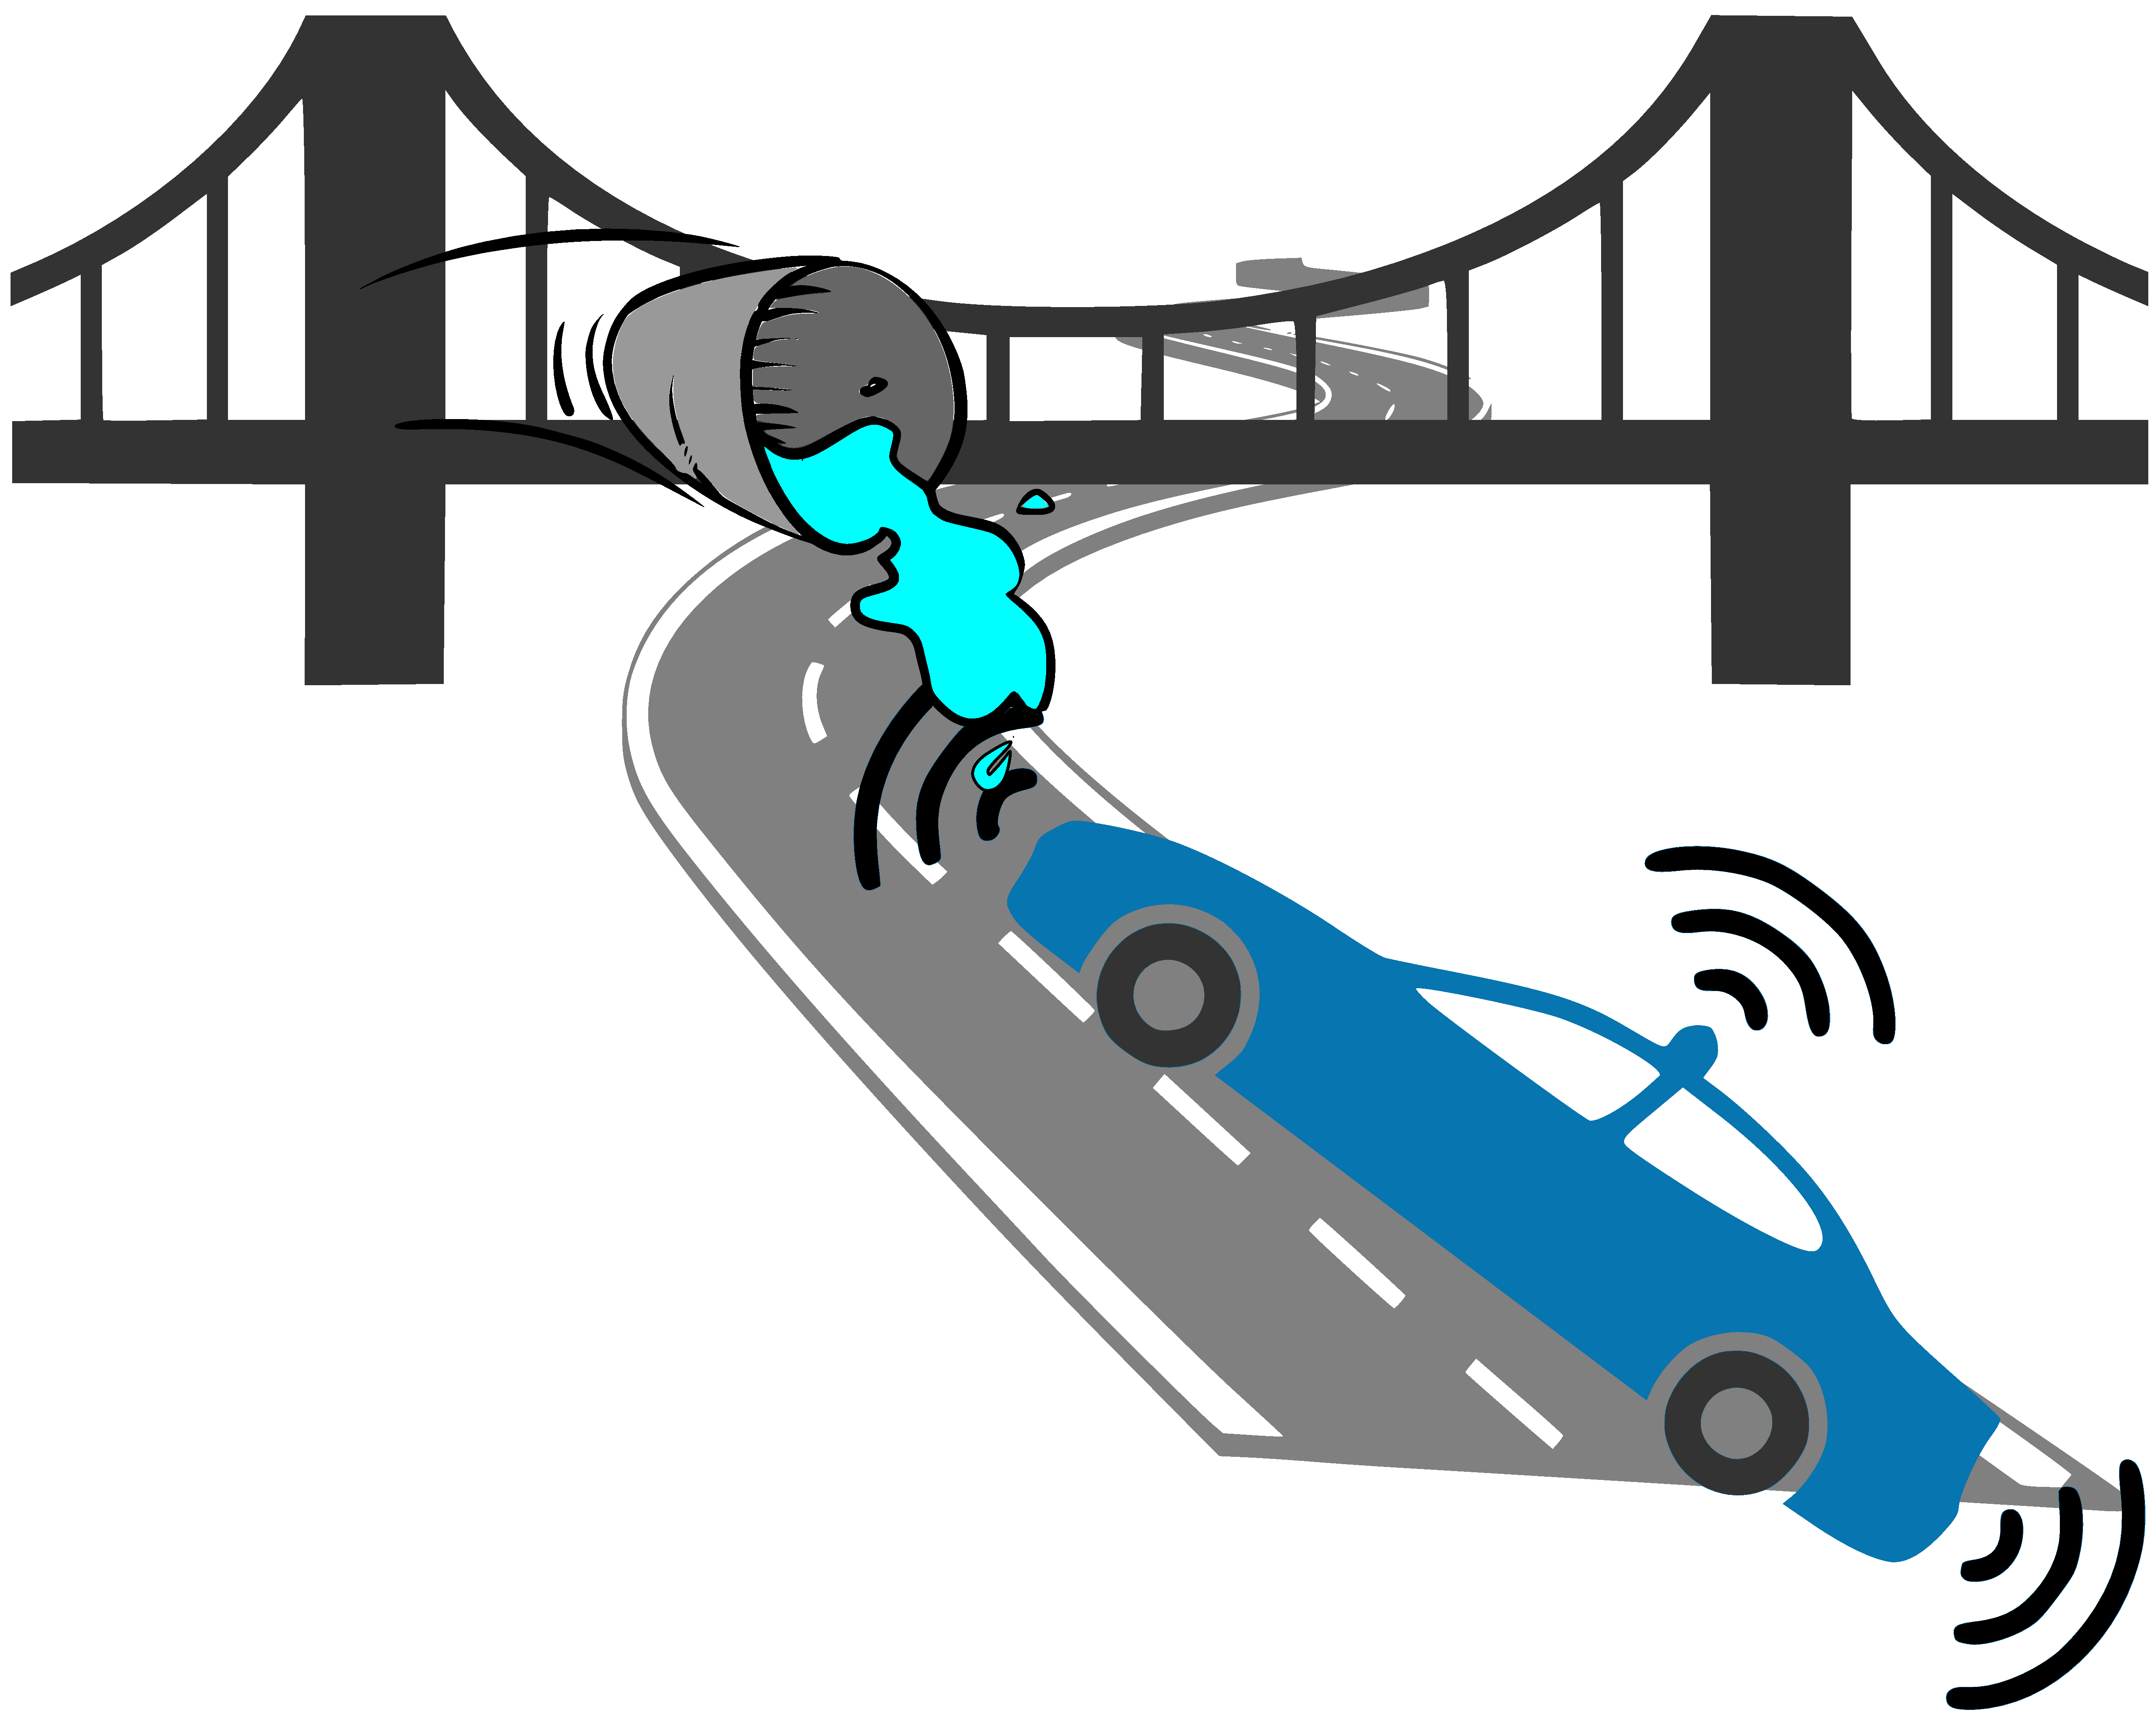
\includegraphics[width=.58\textwidth]{img/bucket-off-bridge.pdf}
	
	
% \end{frame}

% \begin{frame}[fragile]{As if it wasn't difficult enough...}
	
% 	\hspace{1cm}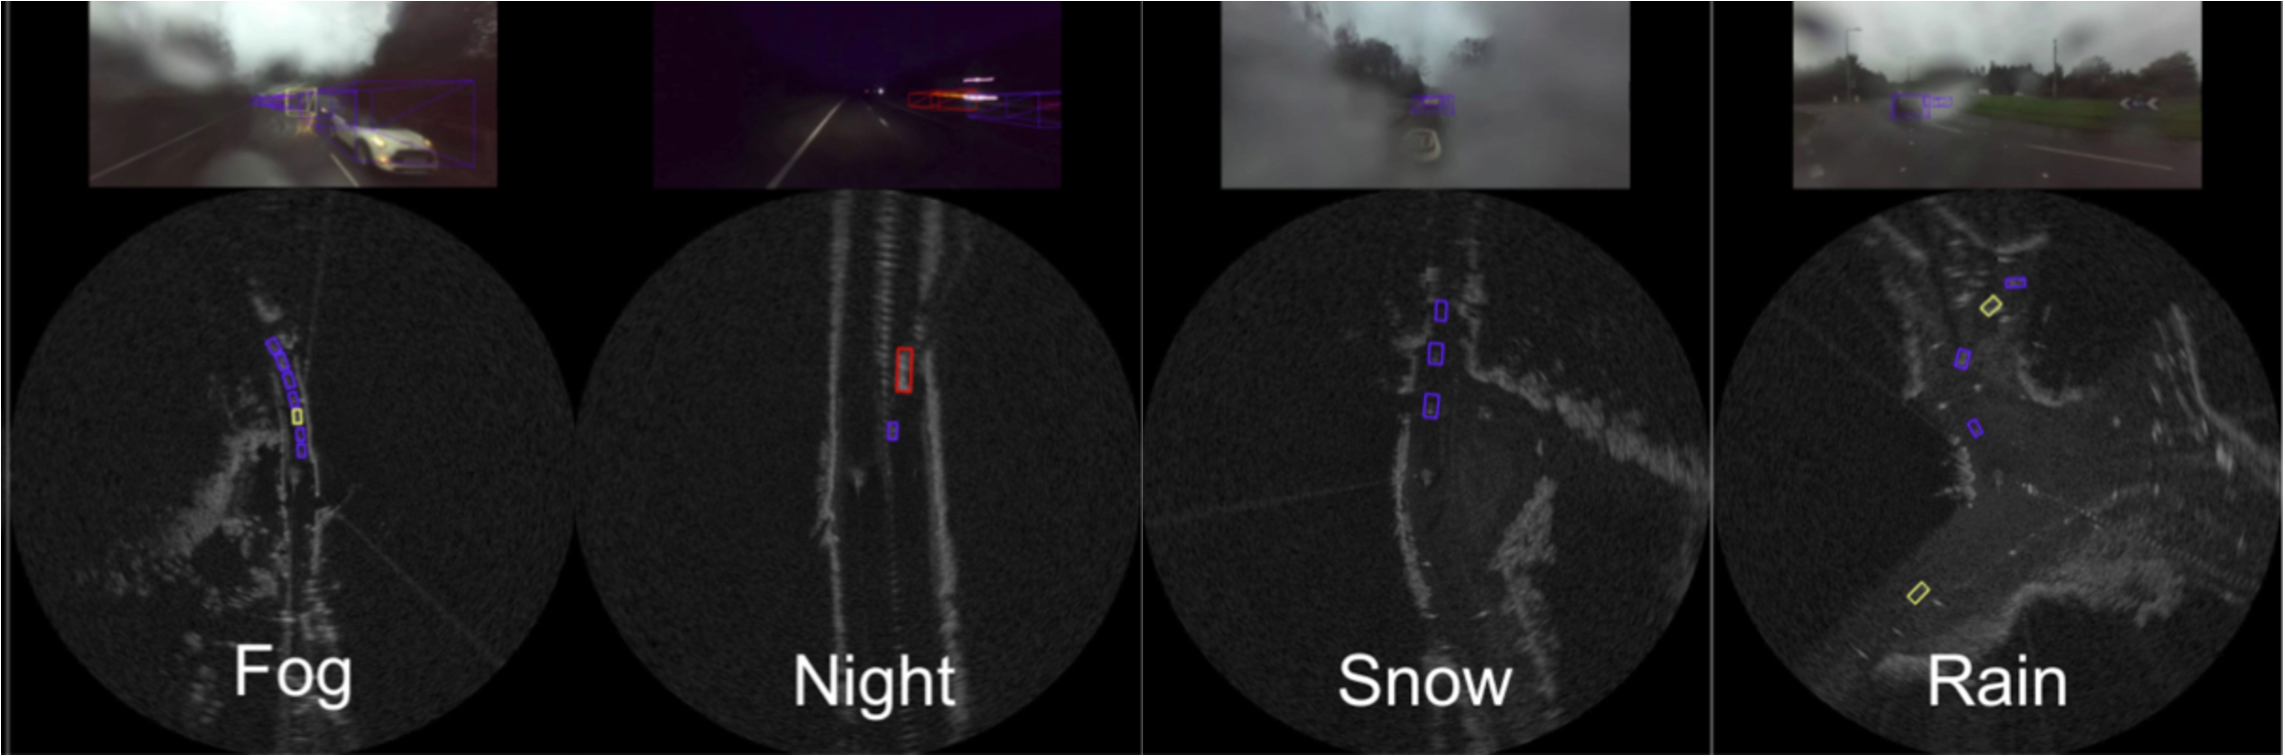
\includegraphics[width=\textwidth]{img/weather2}
	
	
% \end{frame}

% \begin{frame}[fragile]{And To Make it worse...\\Standards Require Safety and Security!}
% 	\vspace{1cm}
% 	\hspace{1cm}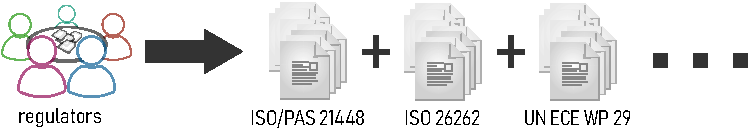
\includegraphics[width=\textwidth]{img/regulations}

	
% \end{frame}

% \begin{frame}[fragile]
% 	%{And To Make it worse...\\Standards Require Safety and Security!}
% 	\vspace{1cm}
% 	%	\hspace{1cm}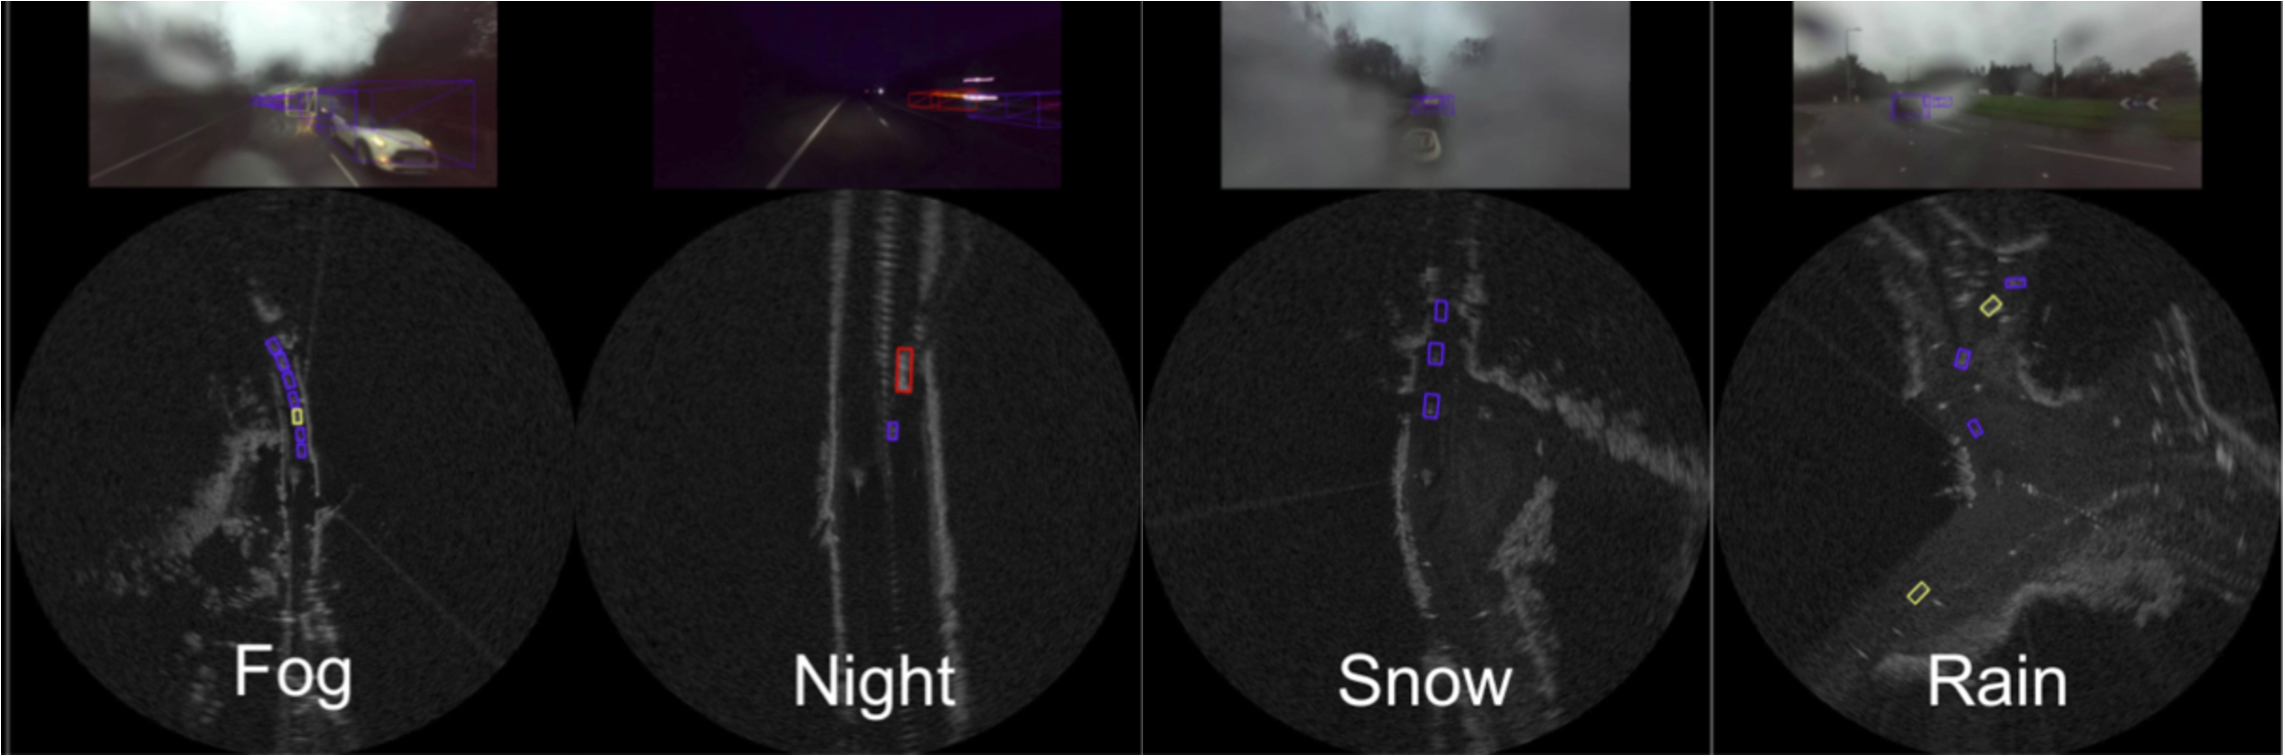
\includegraphics[width=\textwidth]{img/weather2}
% \centering	\Huge{\textcolor{aisecred}{\textbf{So are we doomed?}}}
	
% \end{frame}


% \begin{frame}[fragile]{What do we want}
% %	\vspace{1cm}
% 	%	\hspace{1cm}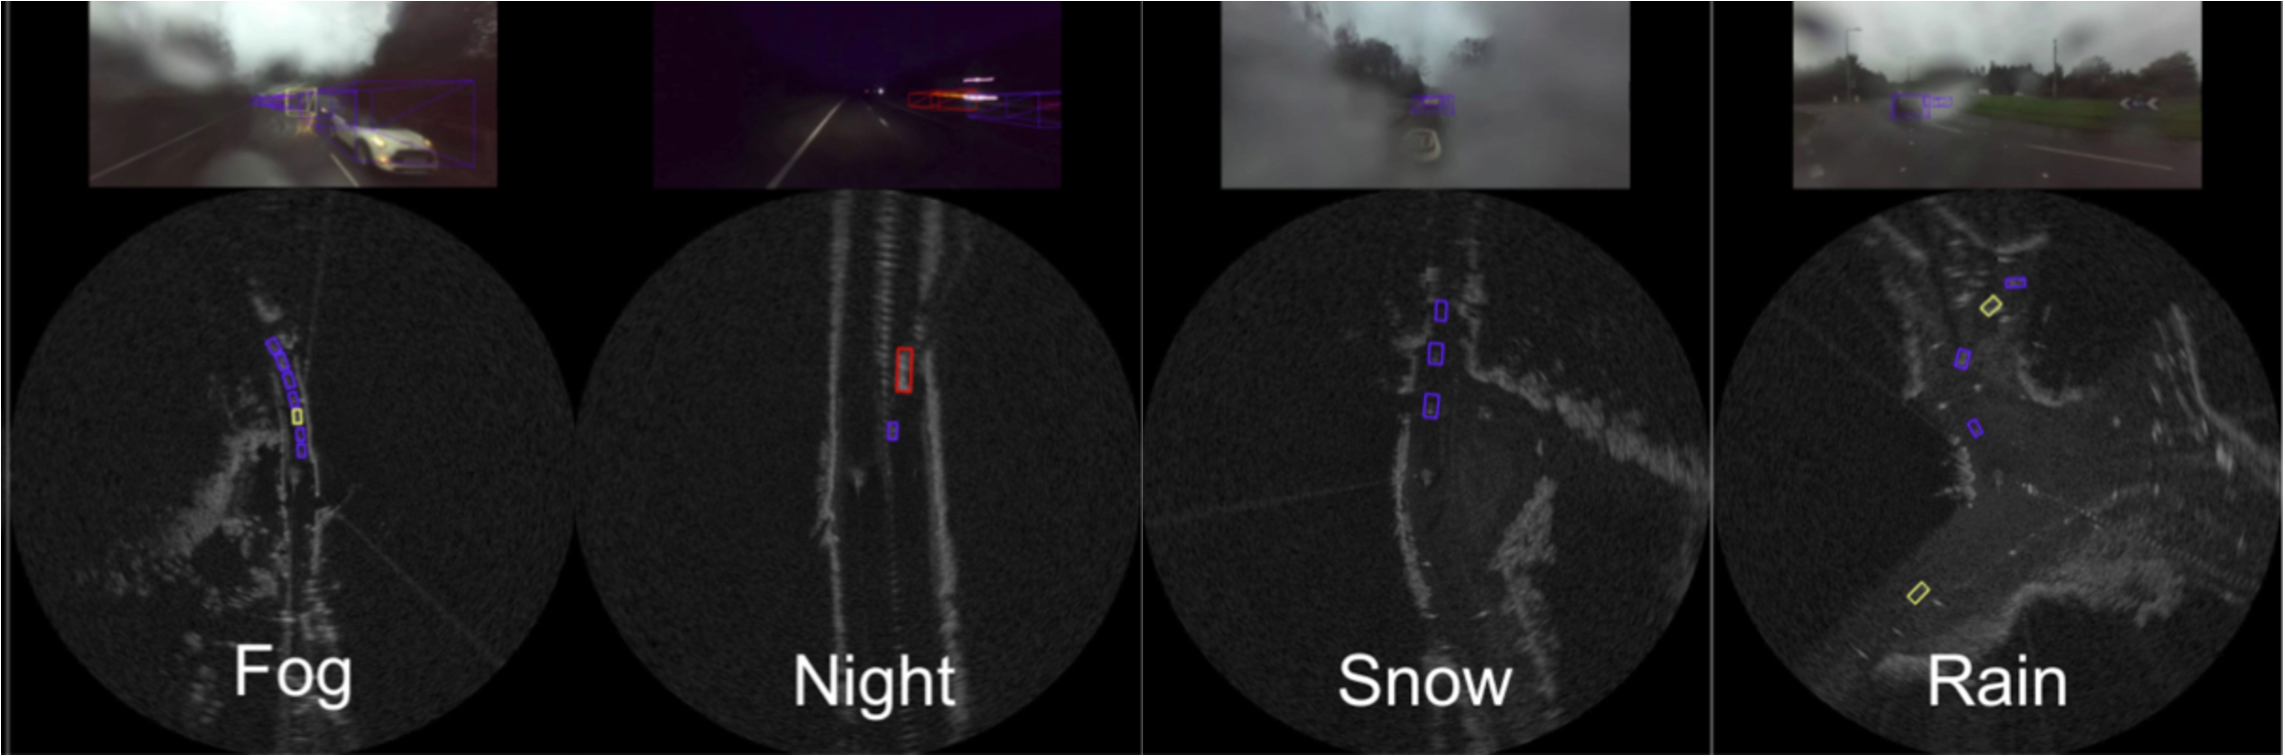
\includegraphics[width=\textwidth]{img/weather2}
	
% 	\Large
% 	\begin{itemize}
% 		\item Guarantees of sensor robustness
% 		\item A certainty around operational domain of safety
% 		\item Protection against attacks
% 	\end{itemize}
	
% 	\vfill
% 	\Huge
% 	\hspace{4cm} ... but how?
% %TODO
% %
% %* guarantees of certain behaviours
% %* a threshold robustness we can work with
% %* protection against attacks
% %* ALL Guaranteed
	
% \end{frame}


% \begin{frame}[fragile]{Formal Verification of ML}
% 	\vspace{-1em}
% 	\begin{alertblock}{Definition of Verification for a Black Box Model}
% 		For a neural network $N : \overline{x} \rightarrow \overline{y}$, the input property $P(\overline{x})$ and the output property $Q(\overline{y})$, does there exist an input $\overline{x_0}$ which satisfies $P(\overline{x_0}$ such that its corresponding output $\overline{y_0}$ satisfies $Q(\overline{y_0})$?
% 	\end{alertblock}
% 		\vspace{-1em}
% 	\begin{itemize}
		
% 		\item $P(\overline{x})$ characterises inputs checked
% 		\item $Q(\overline{y})$ characterises the behaviour we \textcolor{aisecred}{DO NOT} wish for
% 		\item if satisfied, counterexample is returned, else property holds
% 		%want to ensure that or a given input $\overline{x_i}$ (which represents our image) and given amount of noise $\delta$, classification remains the same
% 		% x whose distance from x_i is at most delta, according to some distance matrix
% 		\item the $P$ for traditional adversarial robustness is $\|\overline{x} - \overline{x_0}\| L_{\infty} \leq \delta$
% 		\item the $Q$ is, $\bigvee_i(\overline{y}[i_0] \leq \overline{y}[i])$, where $\overline{y}[i_0]$ is the desired label
% 	\end{itemize}
% %Given an input, potential perturbations to the input (water, light, postit) and a set of outputs, we guaranteee that the outputs cannot change.
% %
% %
% %Now thats something
	
% \end{frame}
\begin{frame}[fragile]{Vehicle Sensor Verification - Reminder}

\begin{alertblock}{Definition of Verification for a Black Box Model}
		For a neural network $N : \hat{x} \rightarrow \hat{y}$, the input property $P(\hat{x})$ and the output property $Q(\hat{y})$, does there exist an input $\hat{x_0}$ which satisfies $P(\hat{x_0})$ such that its corresponding output $\hat{y_0}$ satisfies $Q(\hat{y_0})$?
	\end{alertblock}
		\vspace{0em}
	\begin{itemize}
		
		\item\textcolor{aisecpurple}{ \textbf{$P(\hat{x})$ characterises inputs checked}}
		\item $Q(\hat{y})$ characterises the behaviour we \textcolor{aisecred}{DO NOT} wish for
		\item if satisfied, counterexample is returned, else property holds
		%want to ensure that or a given input $\overline{x_i}$ (which represents our image) and given amount of noise $\delta$, classification remains the same
		% x whose distance from x_i is at most delta, according to some distance matrix
		\item the $P$ for traditional adversarial robustness is $|\hat{x} - \hat{x_0}|_{L_{\infty}} \leq \epsilon$
		\item the $Q$ is, $\bigvee_i(\hat{y}[i_0] \leq \hat{y}[i])$, where $\hat{y}[i_0]$ is the desired label
	\end{itemize}
%Given an input, potential perturbations to the input (water, light, postit) and a set of outputs, we guaranteee that the outputs cannot change.
%
%
%Now thats something
	\end{frame}

\begin{frame}[fragile]{Formal Verification of ML/Sensors - For Resilient Autonomy}
%	\vspace{1cm}
%	If we can guarantee security and safety within a certain range e.g. image of sign, with droplets on it
%	
%	extract the droplets
%	
%	perturbate the droplets
%	
%	Guaranteed safety
%	
%	now thats somethign

\vspace{-0.2em}

\centering\includegraphics[width=0.95\textwidth]{img/guarantee-weather}
	
\end{frame}

\begin{frame}[fragile]{Formally Verified IDS Systems}
    \begin{itemize}
        \item Identification fields: Src IP, Src Port, Dst IP,Dst Port, Protocol,Timestamp
        \item Features: Flow Duration, Fwd/Bwd Header Length, (Fwd/Bwd) Packet Length Min/Max/Mean/Std/Total, Total Fwd/Bwd Packets, (Fwd/Bwd) Inter- Arrival Time Min/Max/Mean/Std/Total, (Fwd/Bwd) SYN/FIN/ACK/RST/CWR/PSH/URG/ECE flags count, Packets/second, Bytes/second, Flow Active Duration Min/Max/Mean/Std, Subflow (Fwd/Bwd) Packets/Bytes, Up/Down Ratio
        \item Label: FlowType (should be mapped to 0 - BENIGN or 1 - MALICIOUS)
        %\item \textbf{\textcolor{aisecred}{Attacker Objective:}} Can packets be manypulated in such a way that the classifcation switches?
         \item \textbf{\textcolor{aisecred}{Objective:}} Given an attacker can perturb these, can we still correctly classify benign and malign traffic?

    \end{itemize}
    
%     \begin{quote}\tiny
% Apruzzese, G., Andreolini, M., Ferretti, L., Marchetti, M., \& Colajanni, M. (2022). Modeling realistic adversarial attacks against network intrusion detection systems. Digital Threats: Research and Practice (DTRAP), 3(3), 1-19.`
% 	 \end{quote}
    

	\begin{quote}
		\tiny Panchuk, B., {Arnaboldi, L.}, Daggitt, L., M., \& Letychevskyi, O. (2023, Coming Soon). Formal Verification of ML Based Network Intrusion Detection. Work in progress
		
	\end{quote}

    
\end{frame}
% \begin{frame}[fragile]{How can we do this}

% \vspace{-1em}

% \begin{quote}
% 	Tool for the verification of security, legal and safety properties 
% 	for AI systems 
% \end{quote}

% \centering 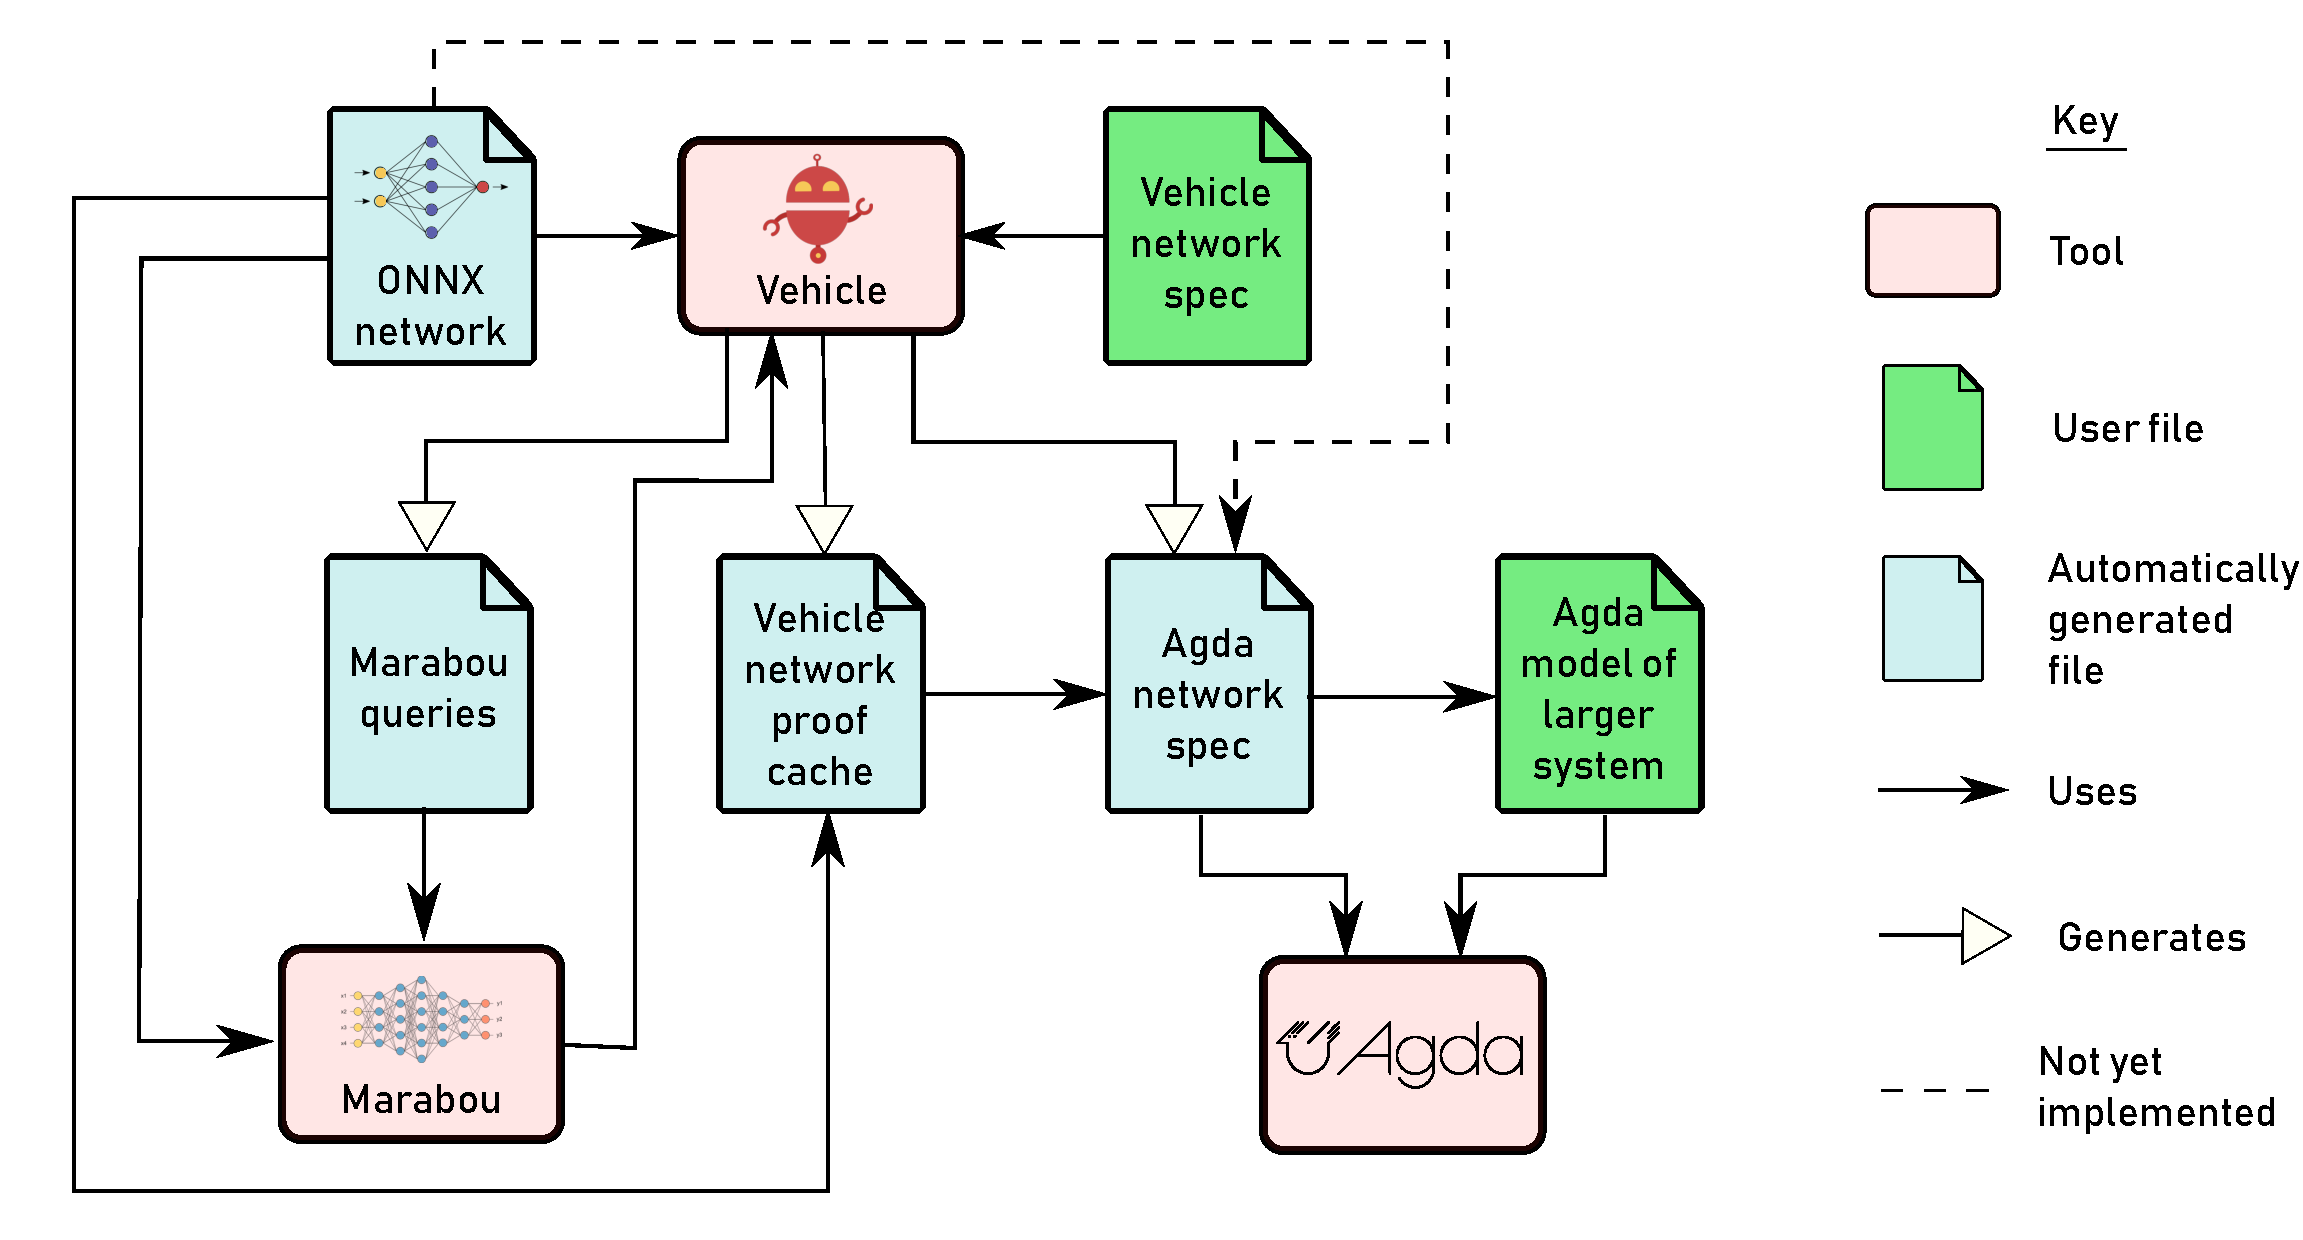
\includegraphics[width=.65\textwidth]{img/architecture.pdf}

% \begin{quote}
% 	\tiny M. Daggitt, W. Kokke, R. Atkey, \textbf{L. Arnaboldi} and E. Komendantskaya (2022) - (Extended Abstract) Vehicle: A High-Level Language for Embedding Logical Specifications in Neural Networks - Workshop on Formal Methods for ML-Enabled Autonomous Systems
% \end{quote}

% \end{frame}
	

\begin{frame}{Vehicle-Tool}{One specification, multiple verifications, and more!}
\centering\vspace{-0.5cm}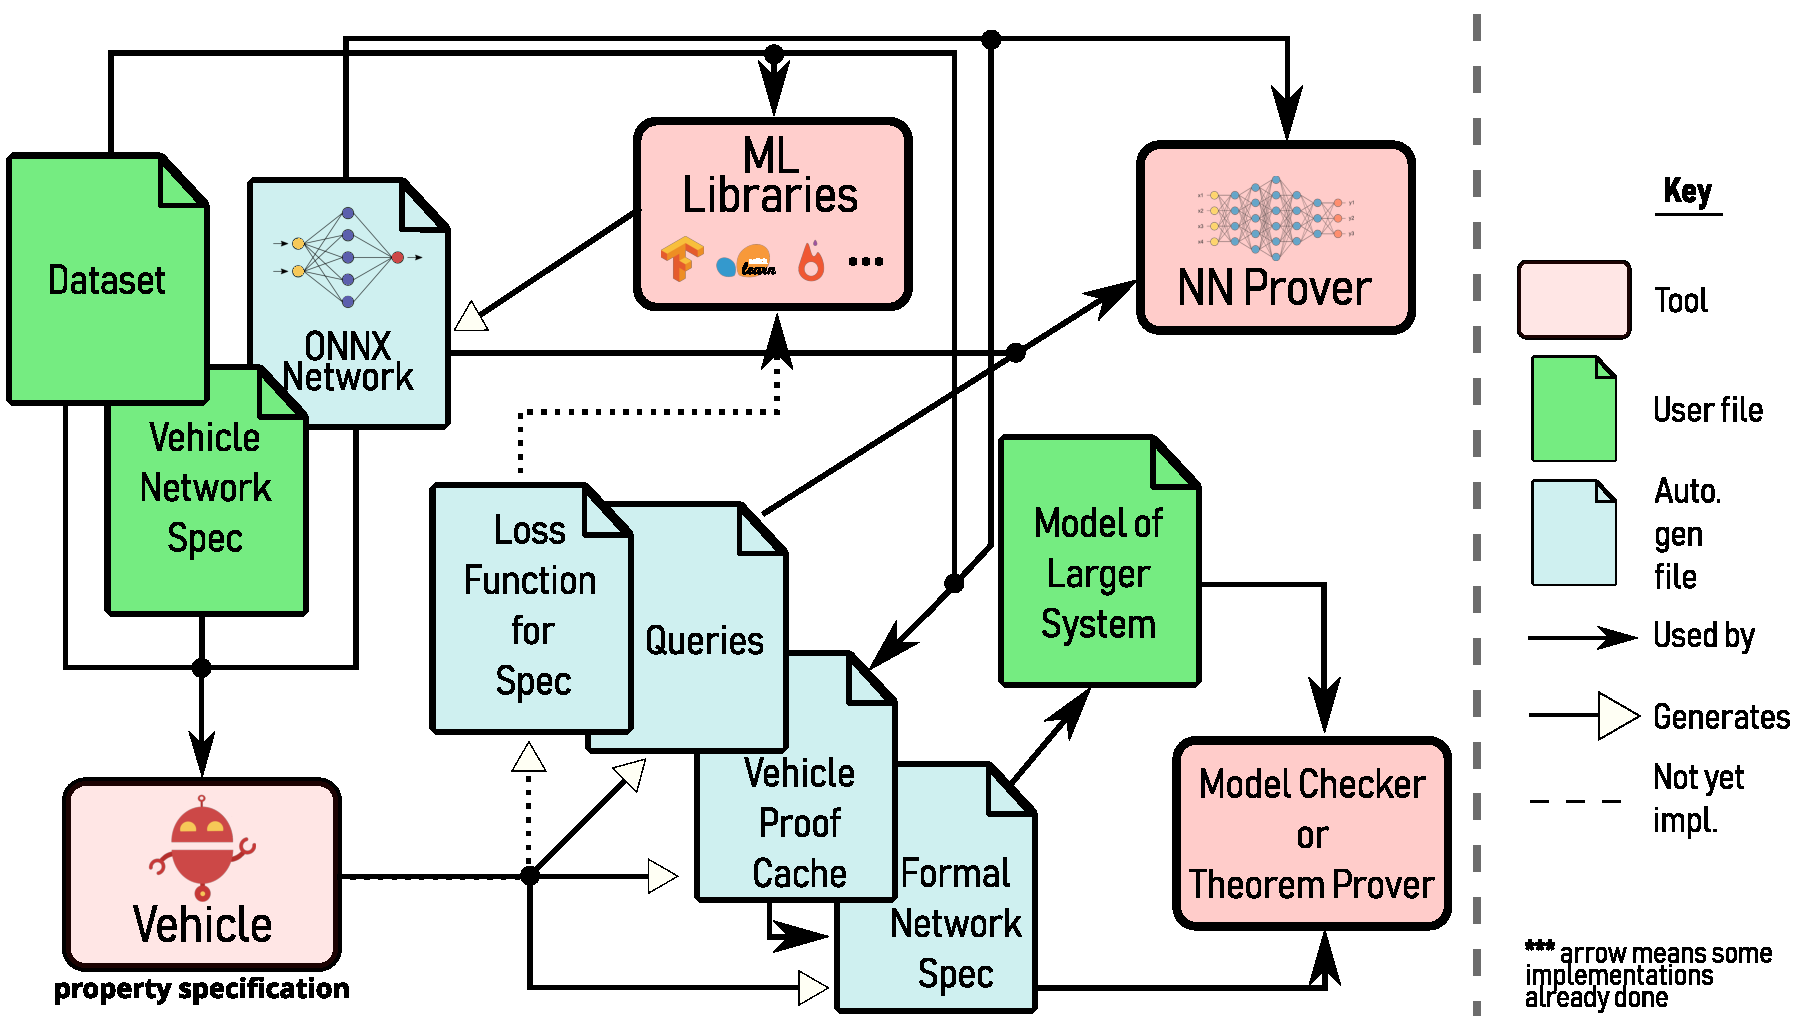
\includegraphics[width=0.8\textwidth]{img/vehicle-overview.pdf}
\end{frame}



% 
\begin{frame}{Conclusions}
	\begin{itemize}
		\item Verification of AI has  tons of security case studies to investigate
        \item Some upcoming research work from the AISEC team:
        \begin{enumerate}
            \item  Create a detailed mathematical representation of different weather events
            \item Formally Verified ML based Network Intrusion Detection
            \item Continue Down NLP path to include Dialogues\\ (e.g. Q. Are you a robot? A. No Q2. Are you sure?)
            \item Formal verification of Soundwaves (e.g. Dolphin Attacks)
        \end{enumerate}

%		\item Let me know if you want 
	\end{itemize}

\vspace{1em}
\Large \centering Thats all folks!

% \vspace{1em}
% \large \centering Interested? Contact me - \  \  \texttt{\textcolor{aisecred}{\faEnvelope\ l.arnaboldi@bham.ac.uk}}
\end{frame}


\end{document}

